\begin{frame}{Making Merger Trees}
    Haloes are defined at distinct snapshots. 
    
    Snapshots correspond to particular values of cosmic time and contain the particle IDs, mass, location $\&$ velocity for each dark matter particle in the simulation.
    
    The aim of a merger tree code is to link clumps (haloes, subhaloes) from an earlier snapshot to the clumps of the consecutive snapshot, i.e. to find the descendants of the clumps of the earlier snapshot within the consecutive snapshot, thus enabling the tracking of growth and merges of haloes in a simulation.
\end{frame}



%{
%    \setbeamertemplate{background}
%    {\vbox to \paperheight{\vfil \hbox to \paperwidth{\hfil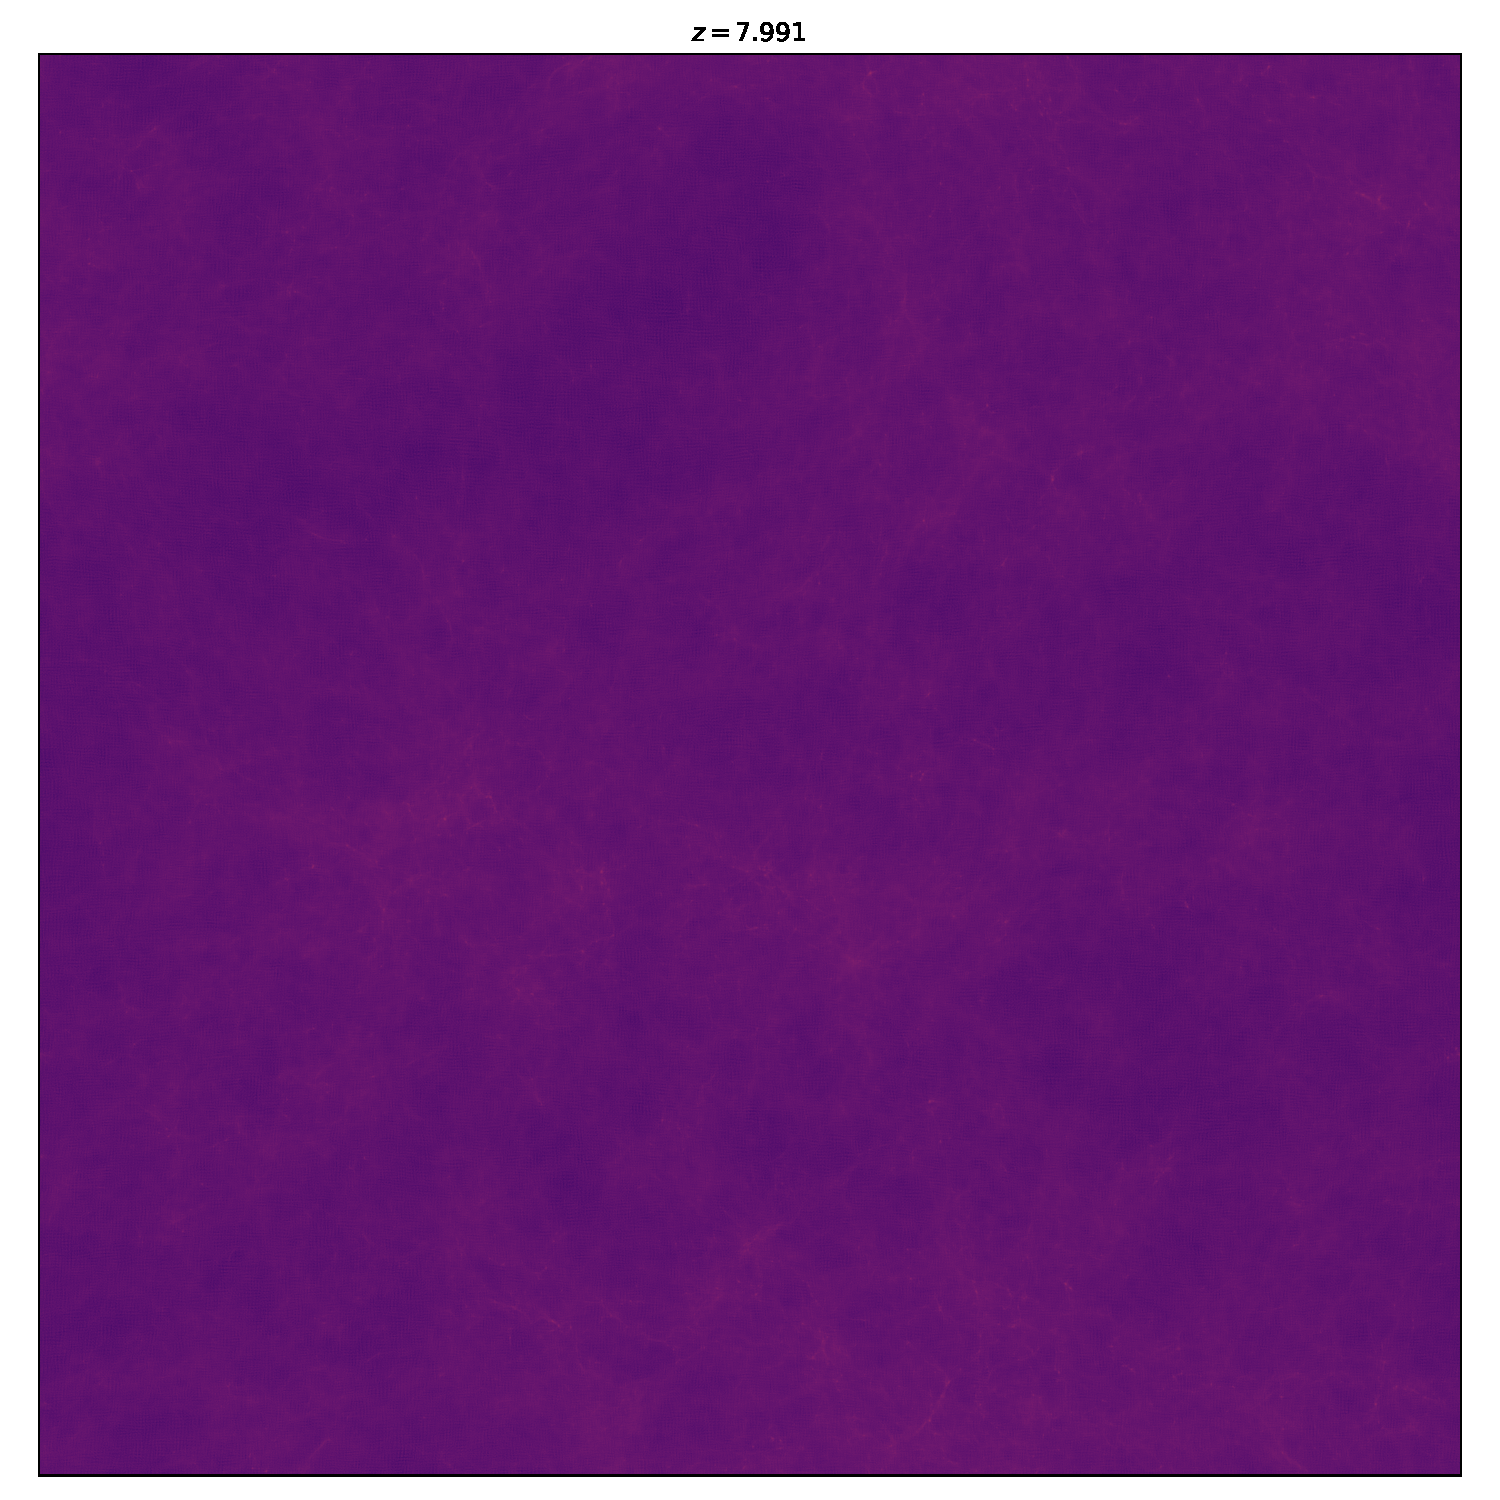
\includegraphics[keepaspectratio,height=\paperheight, width=\paperwidth]{./images/snapshots/particleplot_00002_nolabels.pdf}\hfil}\vfil}}
%    \begin{frame}[plain]
%    \end{frame}
%}
%{
%    \setbeamertemplate{background}
%    {\vbox to \paperheight{\vfil \hbox to \paperwidth{\hfil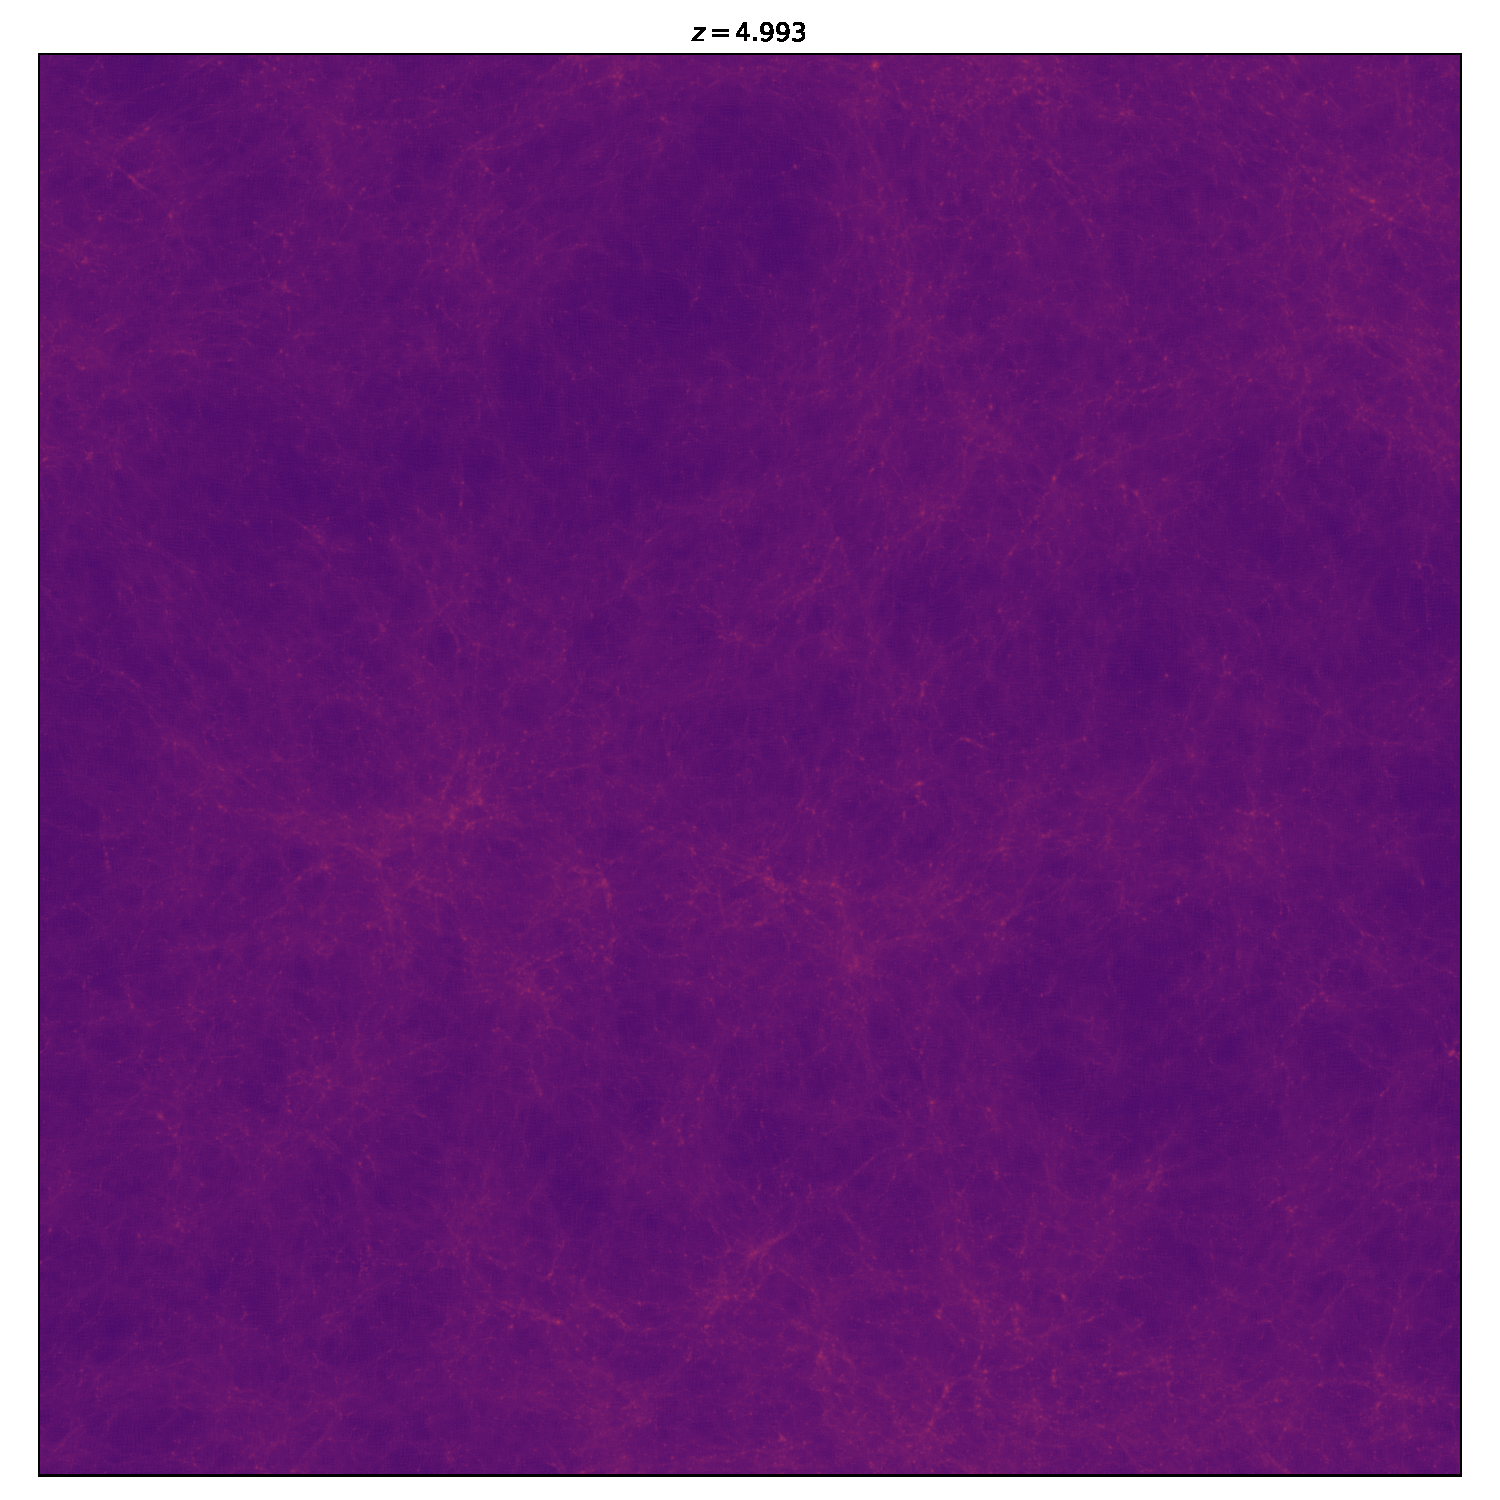
\includegraphics[keepaspectratio,height=\paperheight, width=\paperwidth]{./images/snapshots/particleplot_00005_nolabels.pdf}\hfil}\vfil}}
%    \begin{frame}[plain]
%    \end{frame}
%}
%{
%    \setbeamertemplate{background}
%    {\vbox to \paperheight{\vfil \hbox to \paperwidth{\hfil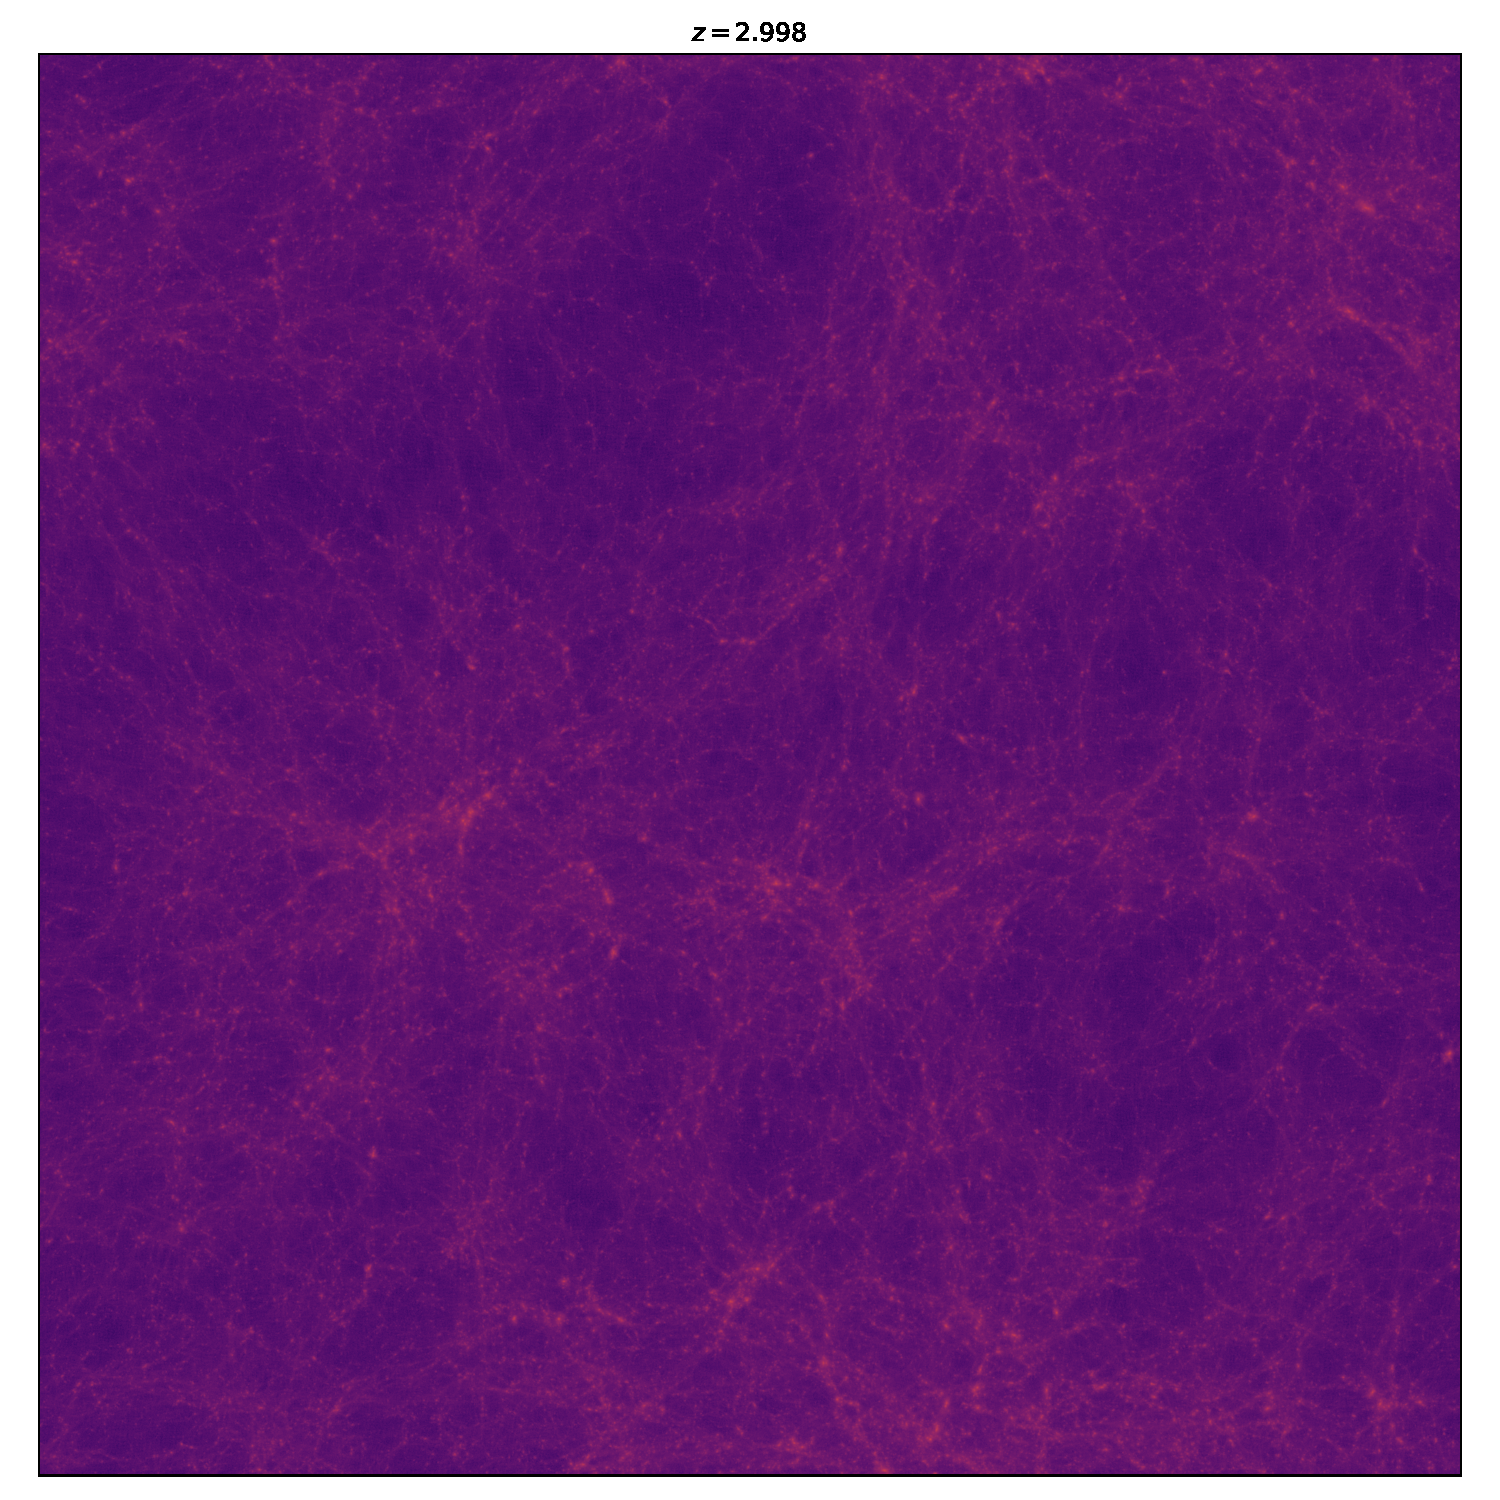
\includegraphics[keepaspectratio,height=\paperheight, width=\paperwidth]{./images/snapshots/particleplot_00008_nolabels.pdf}\hfil}\vfil}}
%    \begin{frame}[plain]
%    \end{frame}
%}
%{
%    \setbeamertemplate{background}
%    {\vbox to \paperheight{\vfil \hbox to \paperwidth{\hfil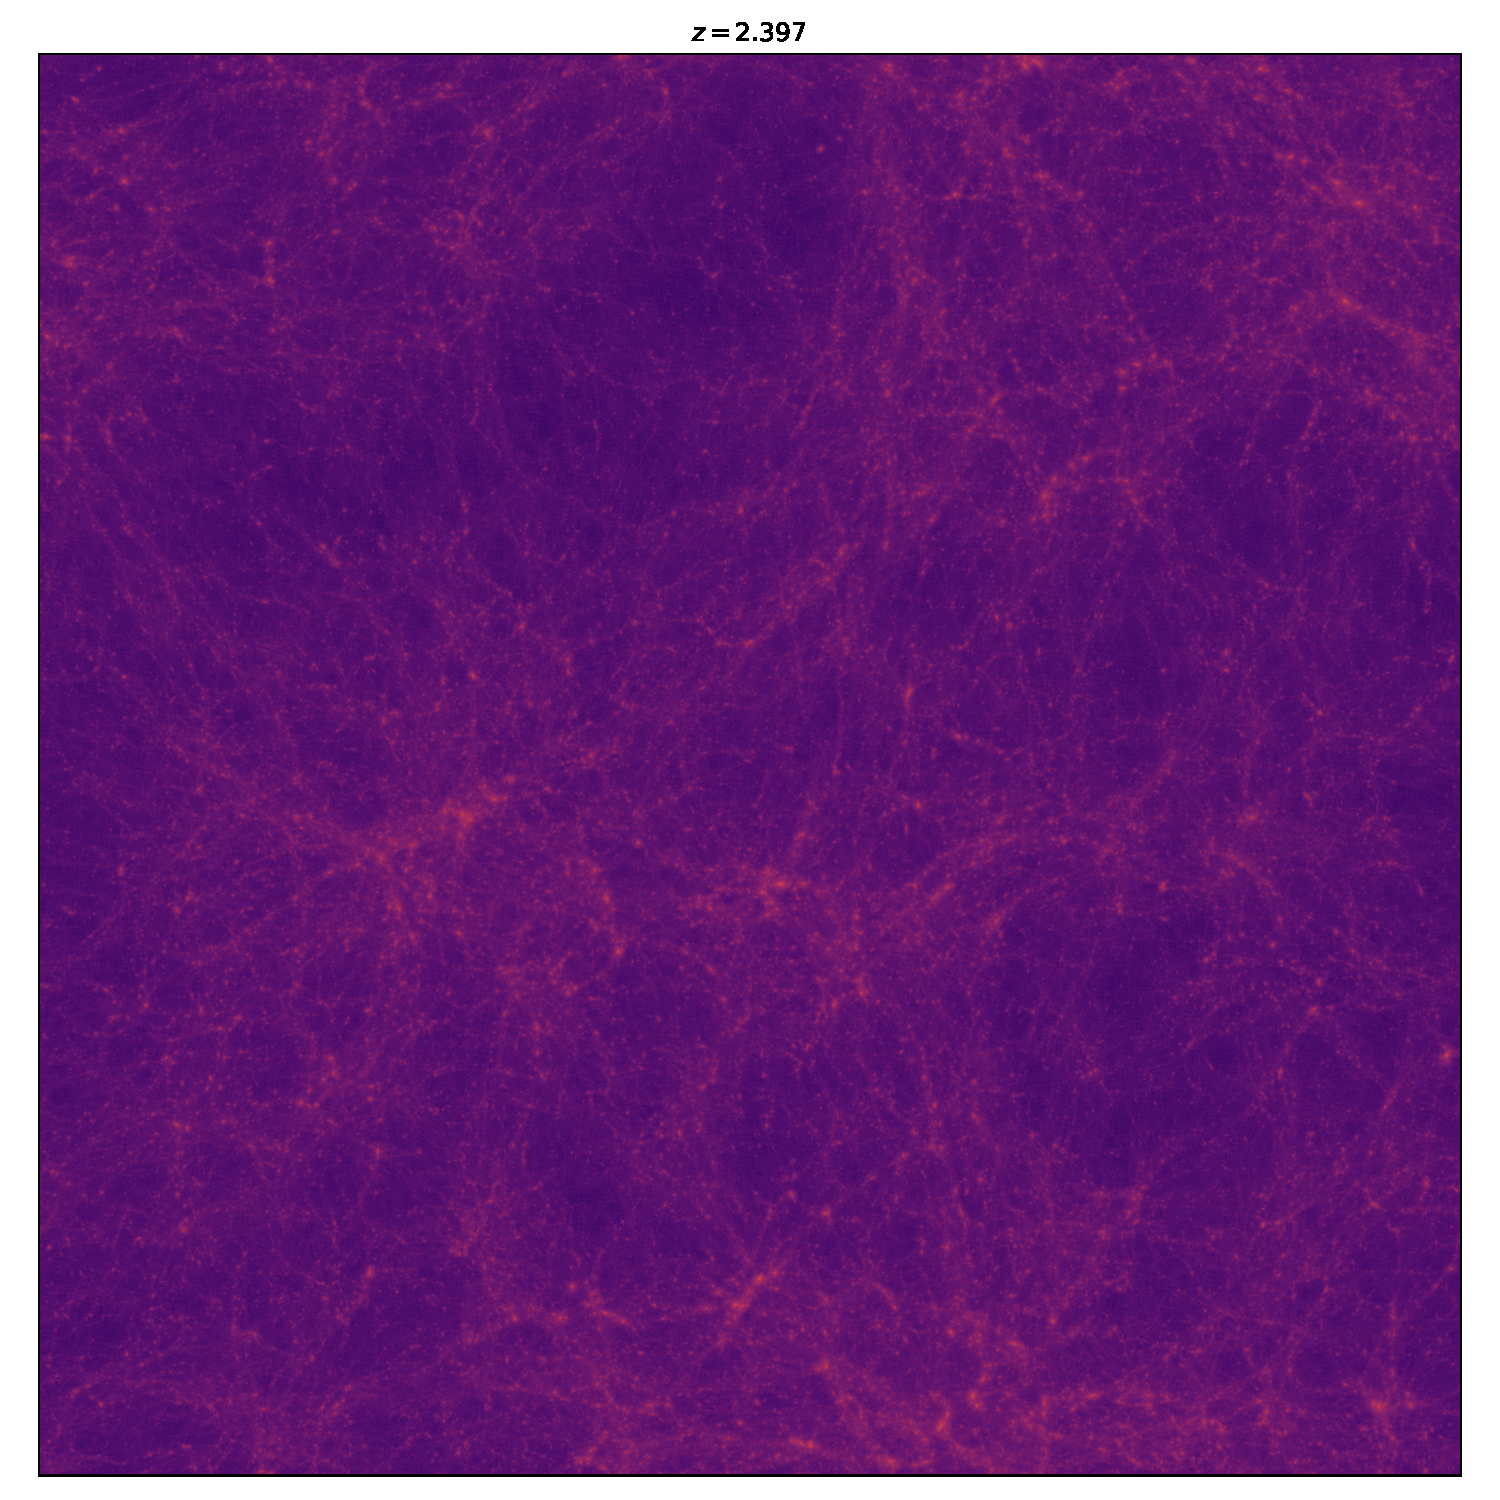
\includegraphics[keepaspectratio,height=\paperheight, width=\paperwidth]{./images/snapshots/particleplot_00011_nolabels.pdf}\hfil}\vfil}}
%    \begin{frame}[plain]
%    \end{frame}
%}
%{
%    \setbeamertemplate{background}
%    {\vbox to \paperheight{\vfil \hbox to \paperwidth{\hfil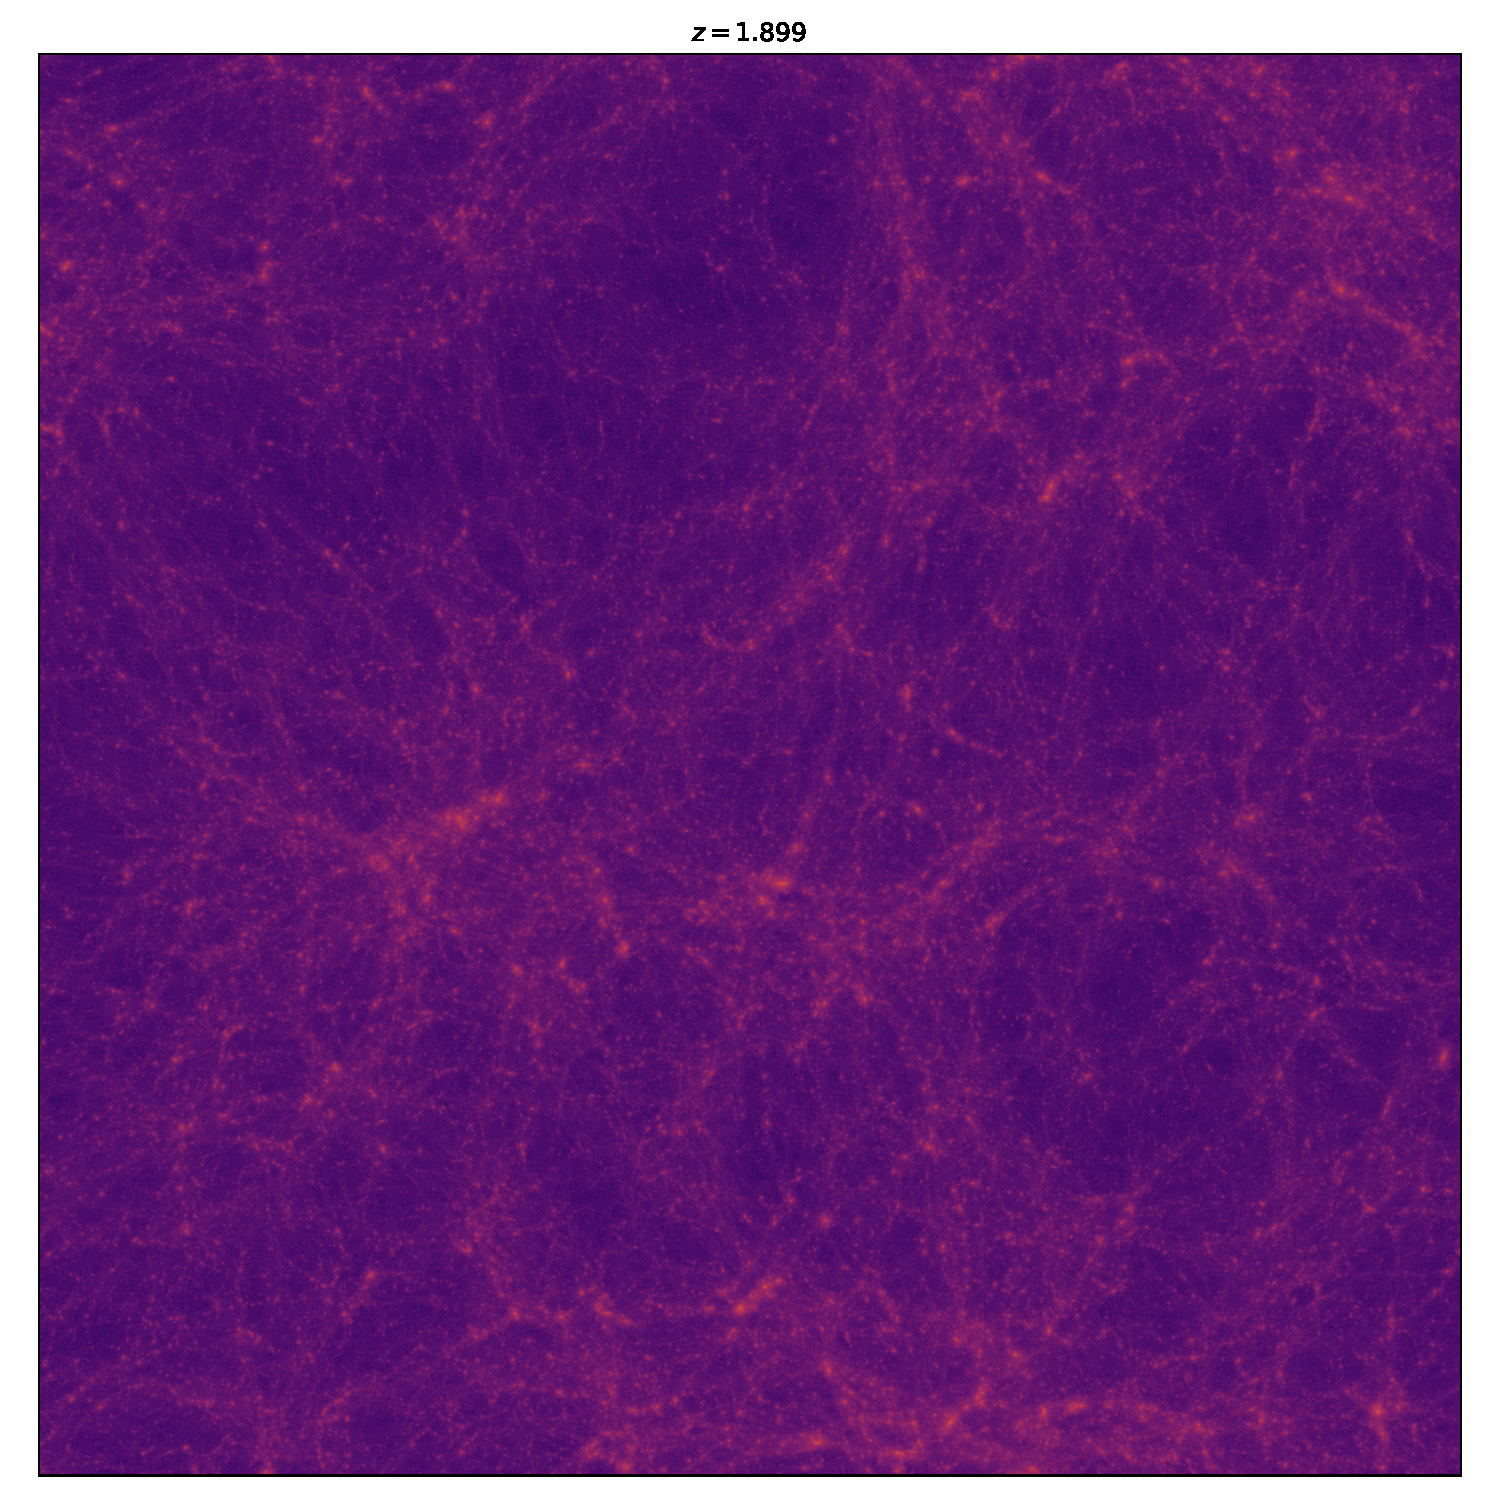
\includegraphics[keepaspectratio,height=\paperheight, width=\paperwidth]{./images/snapshots/particleplot_00014_nolabels.pdf}\hfil}\vfil}}
%    \begin{frame}[plain]
%    \end{frame}
%}
%{
%    \setbeamertemplate{background}
%    {\vbox to \paperheight{\vfil \hbox to \paperwidth{\hfil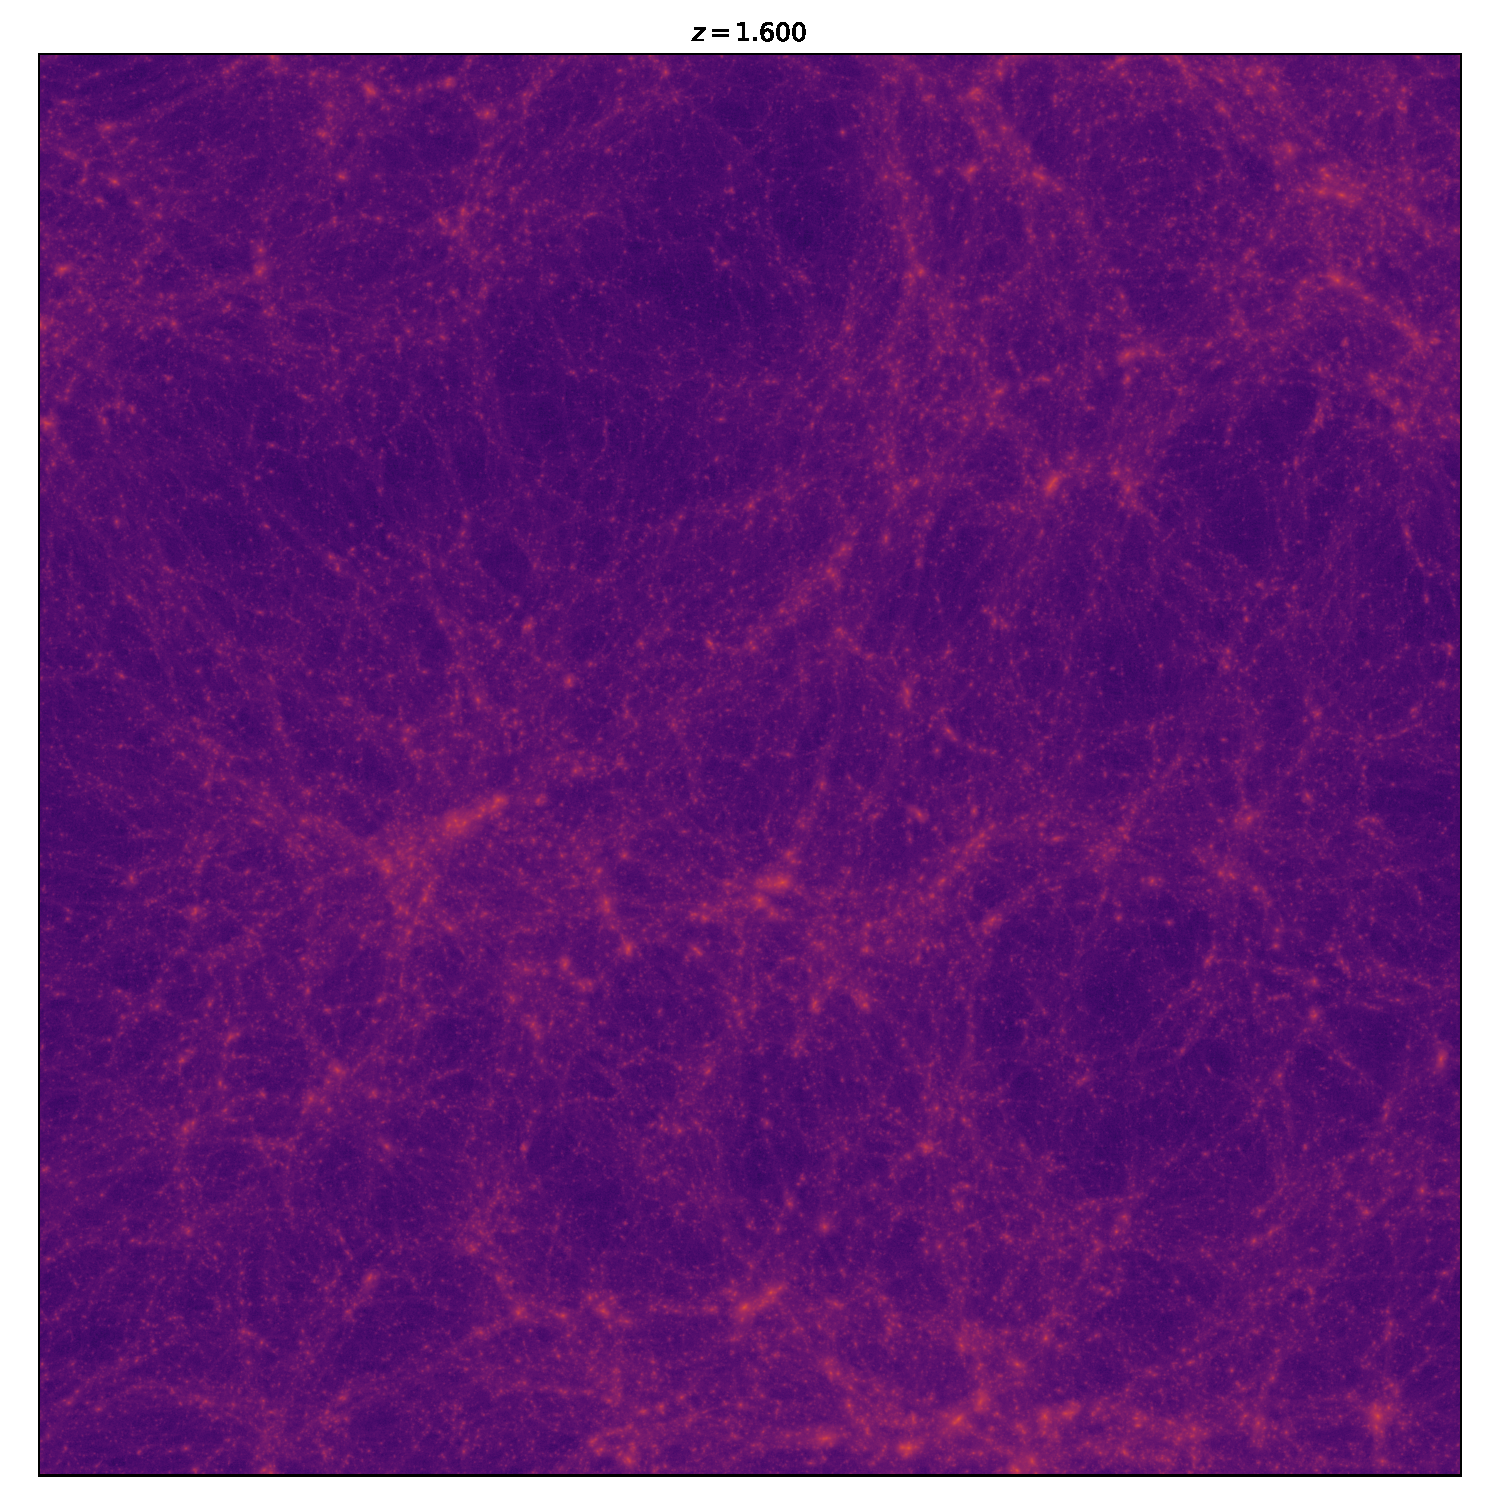
\includegraphics[keepaspectratio,height=\paperheight, width=\paperwidth]{./images/snapshots/particleplot_00017_nolabels.pdf}\hfil}\vfil}}
%    \begin{frame}[plain]
%    \end{frame}
%}
%{
%    \setbeamertemplate{background}
%    {\vbox to \paperheight{\vfil \hbox to \paperwidth{\hfil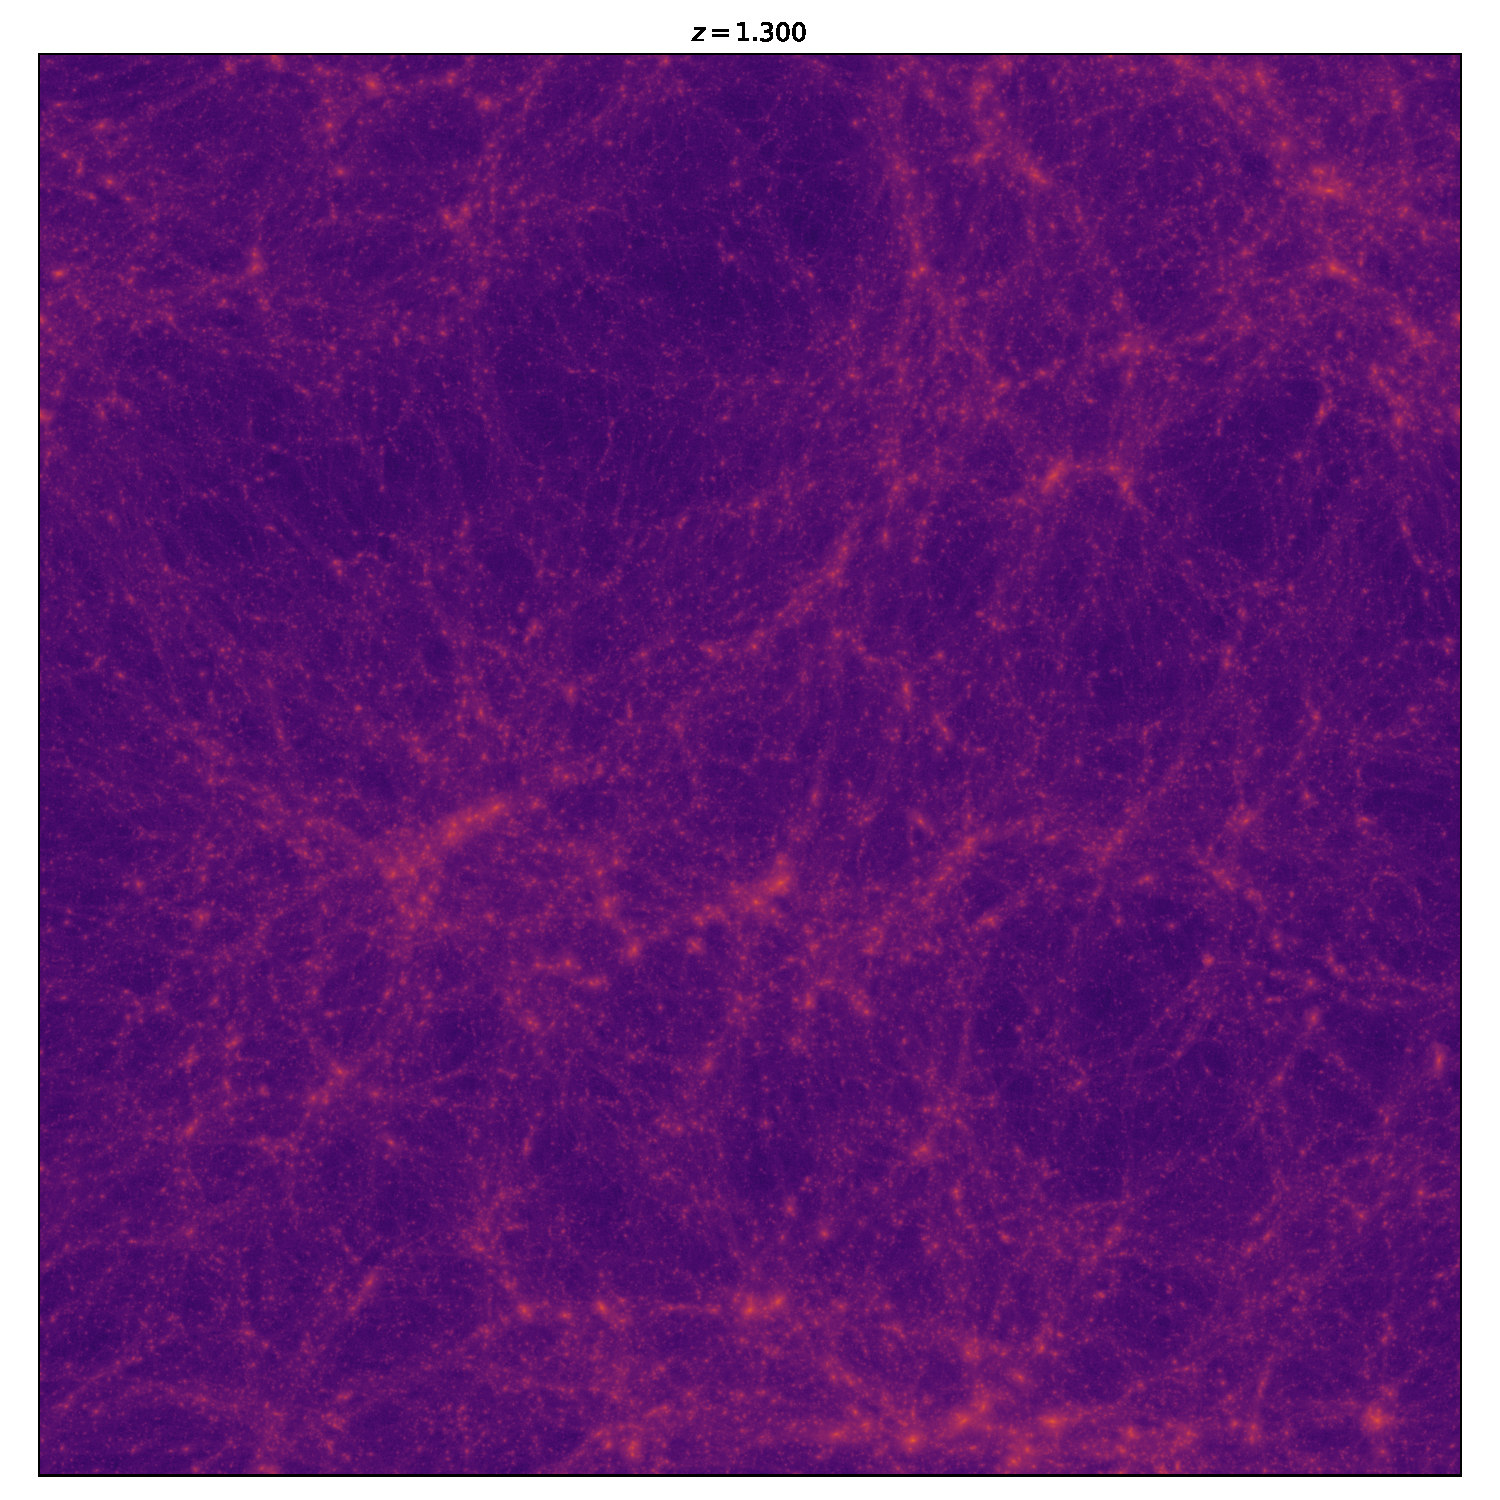
\includegraphics[keepaspectratio,height=\paperheight, width=\paperwidth]{./images/snapshots/particleplot_00020_nolabels.pdf}\hfil}\vfil}}
%    \begin{frame}[plain]
%    \end{frame}
%}
%{
%    \setbeamertemplate{background}
%    {\vbox to \paperheight{\vfil \hbox to \paperwidth{\hfil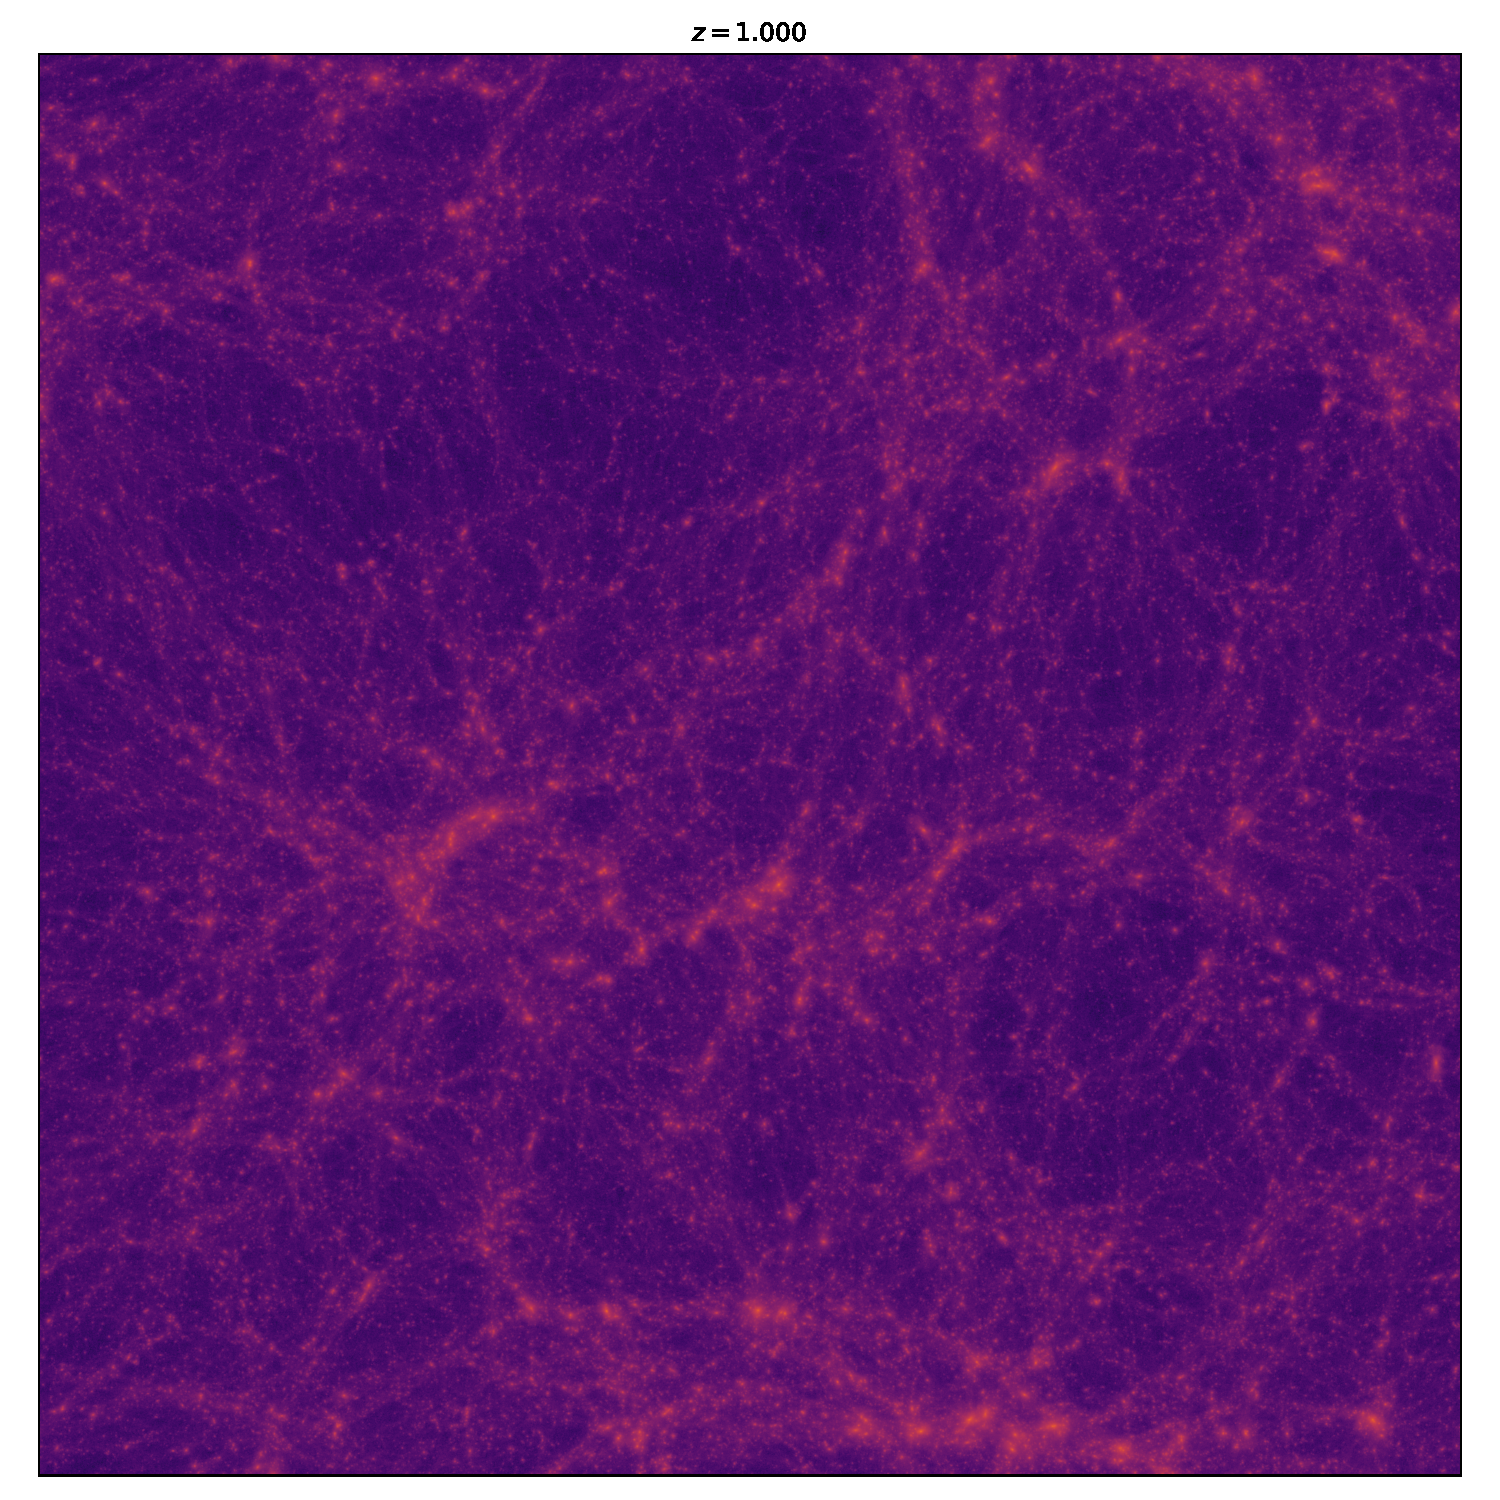
\includegraphics[keepaspectratio,height=\paperheight, width=\paperwidth]{./images/snapshots/particleplot_00023_nolabels.pdf}\hfil}\vfil}}
%    \begin{frame}[plain]
%    \end{frame}
%}
%{
%    \setbeamertemplate{background}
%    {\vbox to \paperheight{\vfil \hbox to \paperwidth{\hfil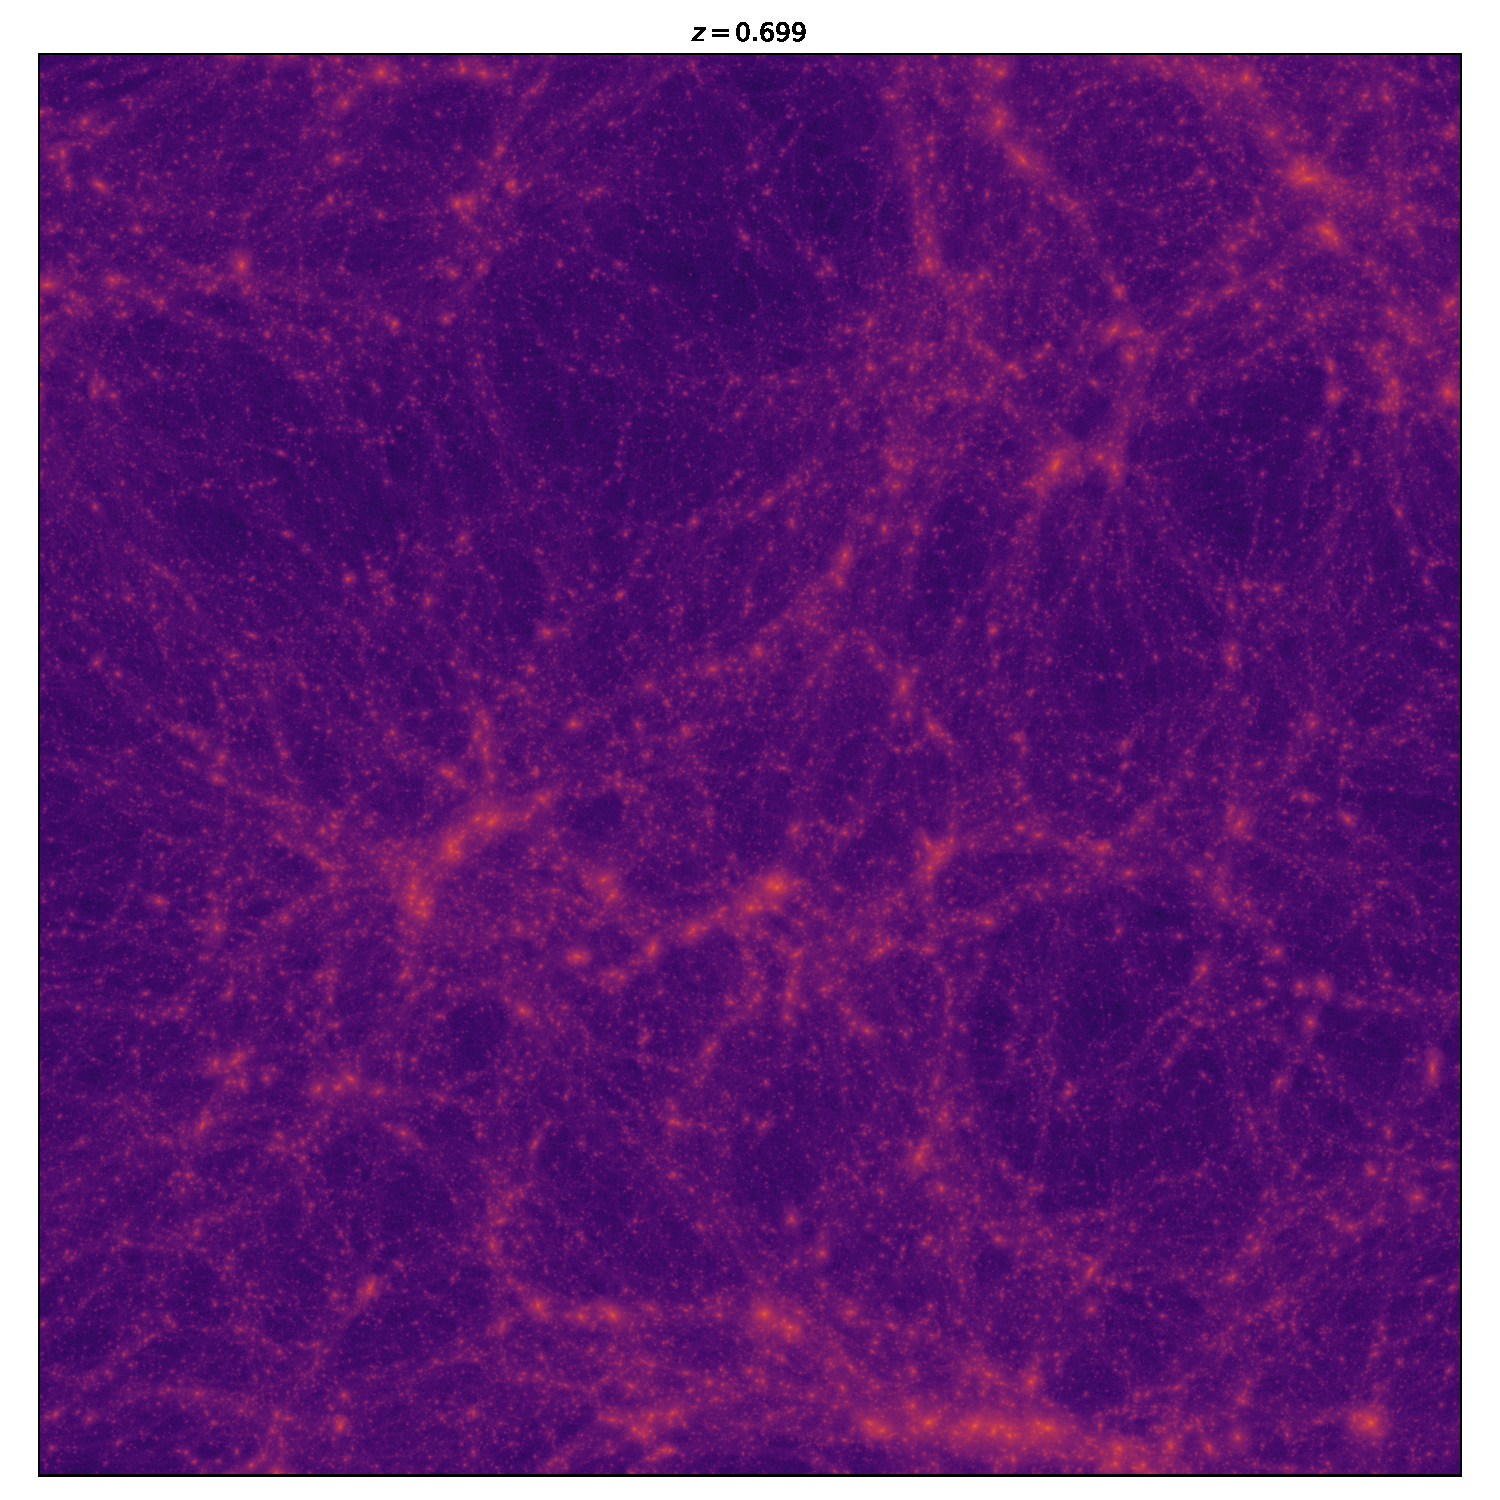
\includegraphics[keepaspectratio,height=\paperheight, width=\paperwidth]{./images/snapshots/particleplot_00026_nolabels.pdf}\hfil}\vfil}}
%    \begin{frame}[plain]
%    \end{frame}
%}
%{
%    \setbeamertemplate{background}
%    {\vbox to \paperheight{\vfil \hbox to \paperwidth{\hfil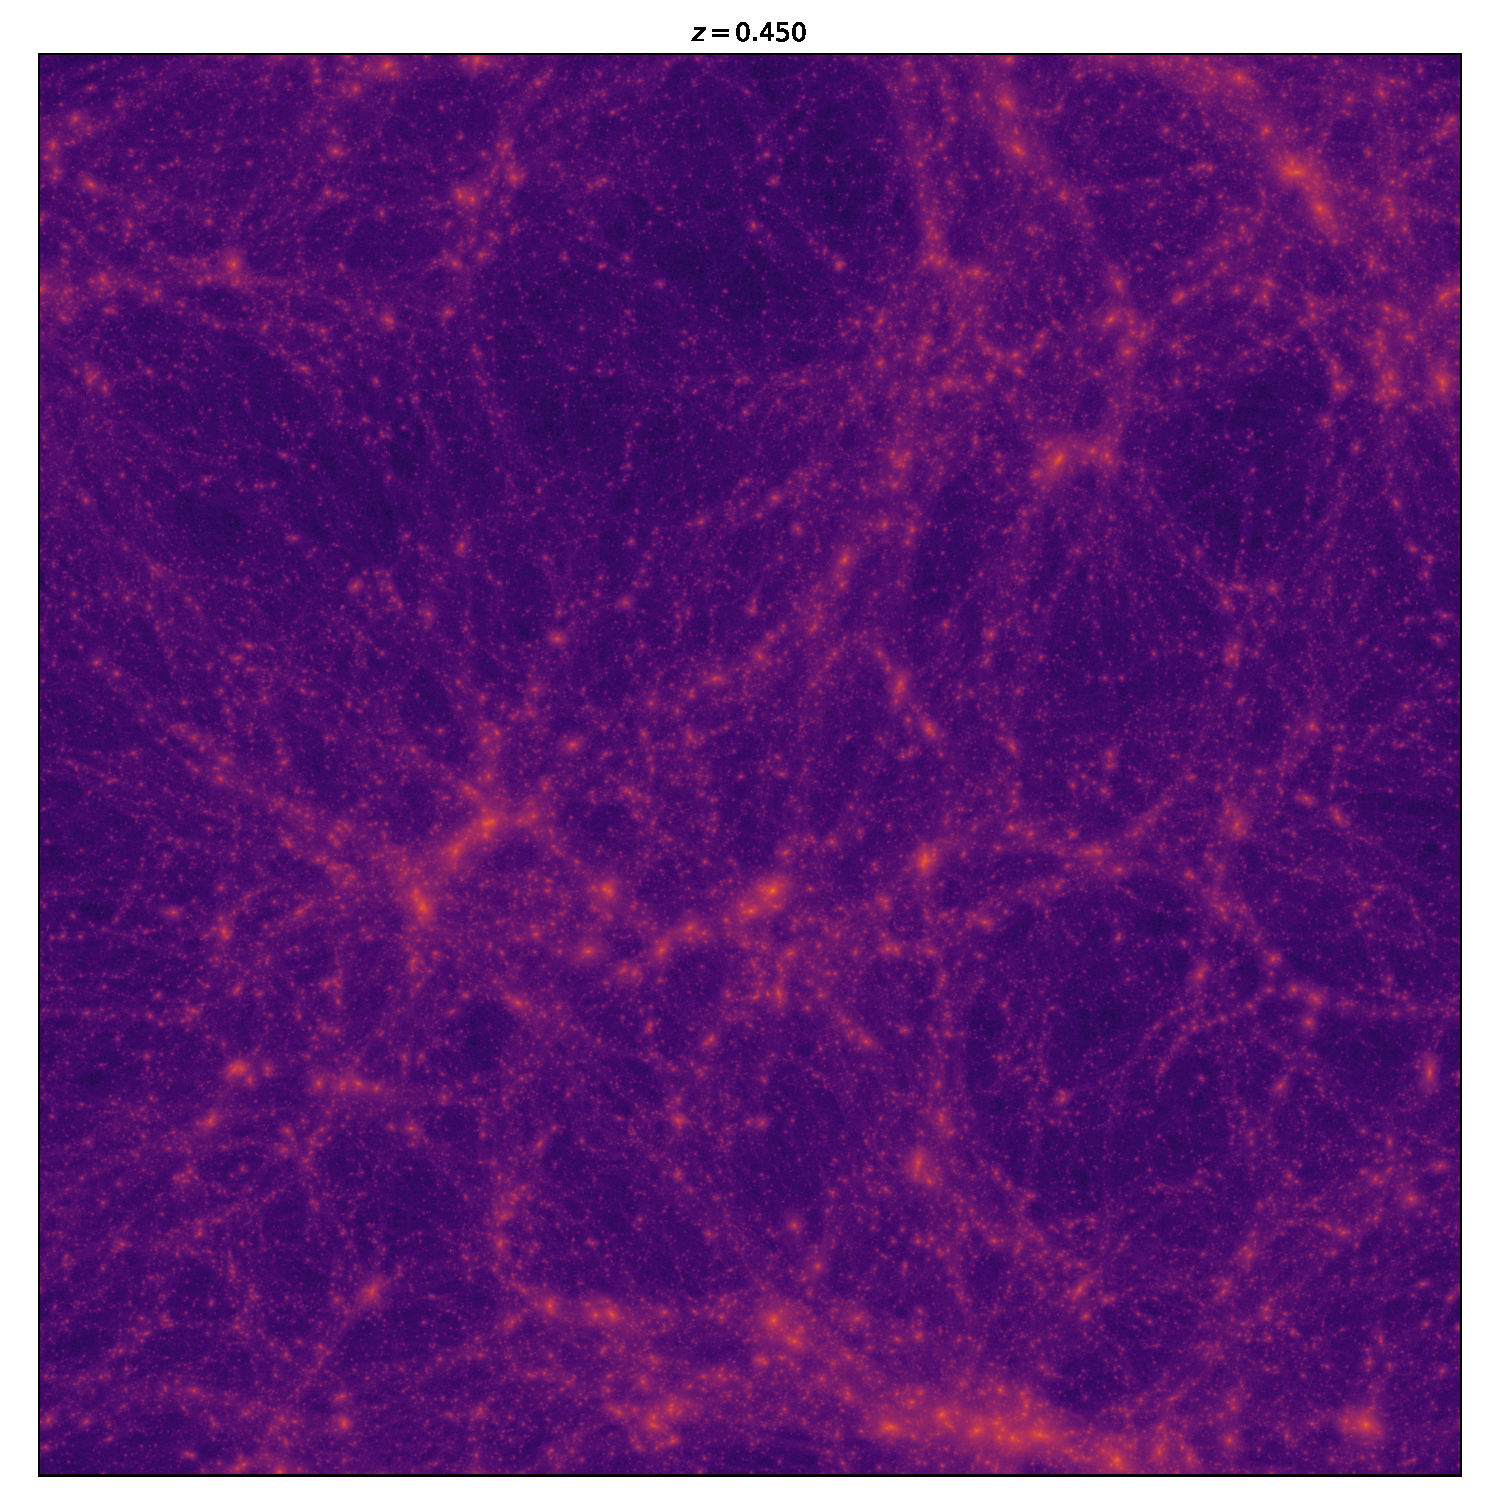
\includegraphics[keepaspectratio,height=\paperheight, width=\paperwidth]{./images/snapshots/particleplot_00029_nolabels.pdf}\hfil}\vfil}}
%    \begin{frame}[plain]
%    \end{frame}
%}
%{
%    \setbeamertemplate{background}
%    {\vbox to \paperheight{\vfil \hbox to \paperwidth{\hfil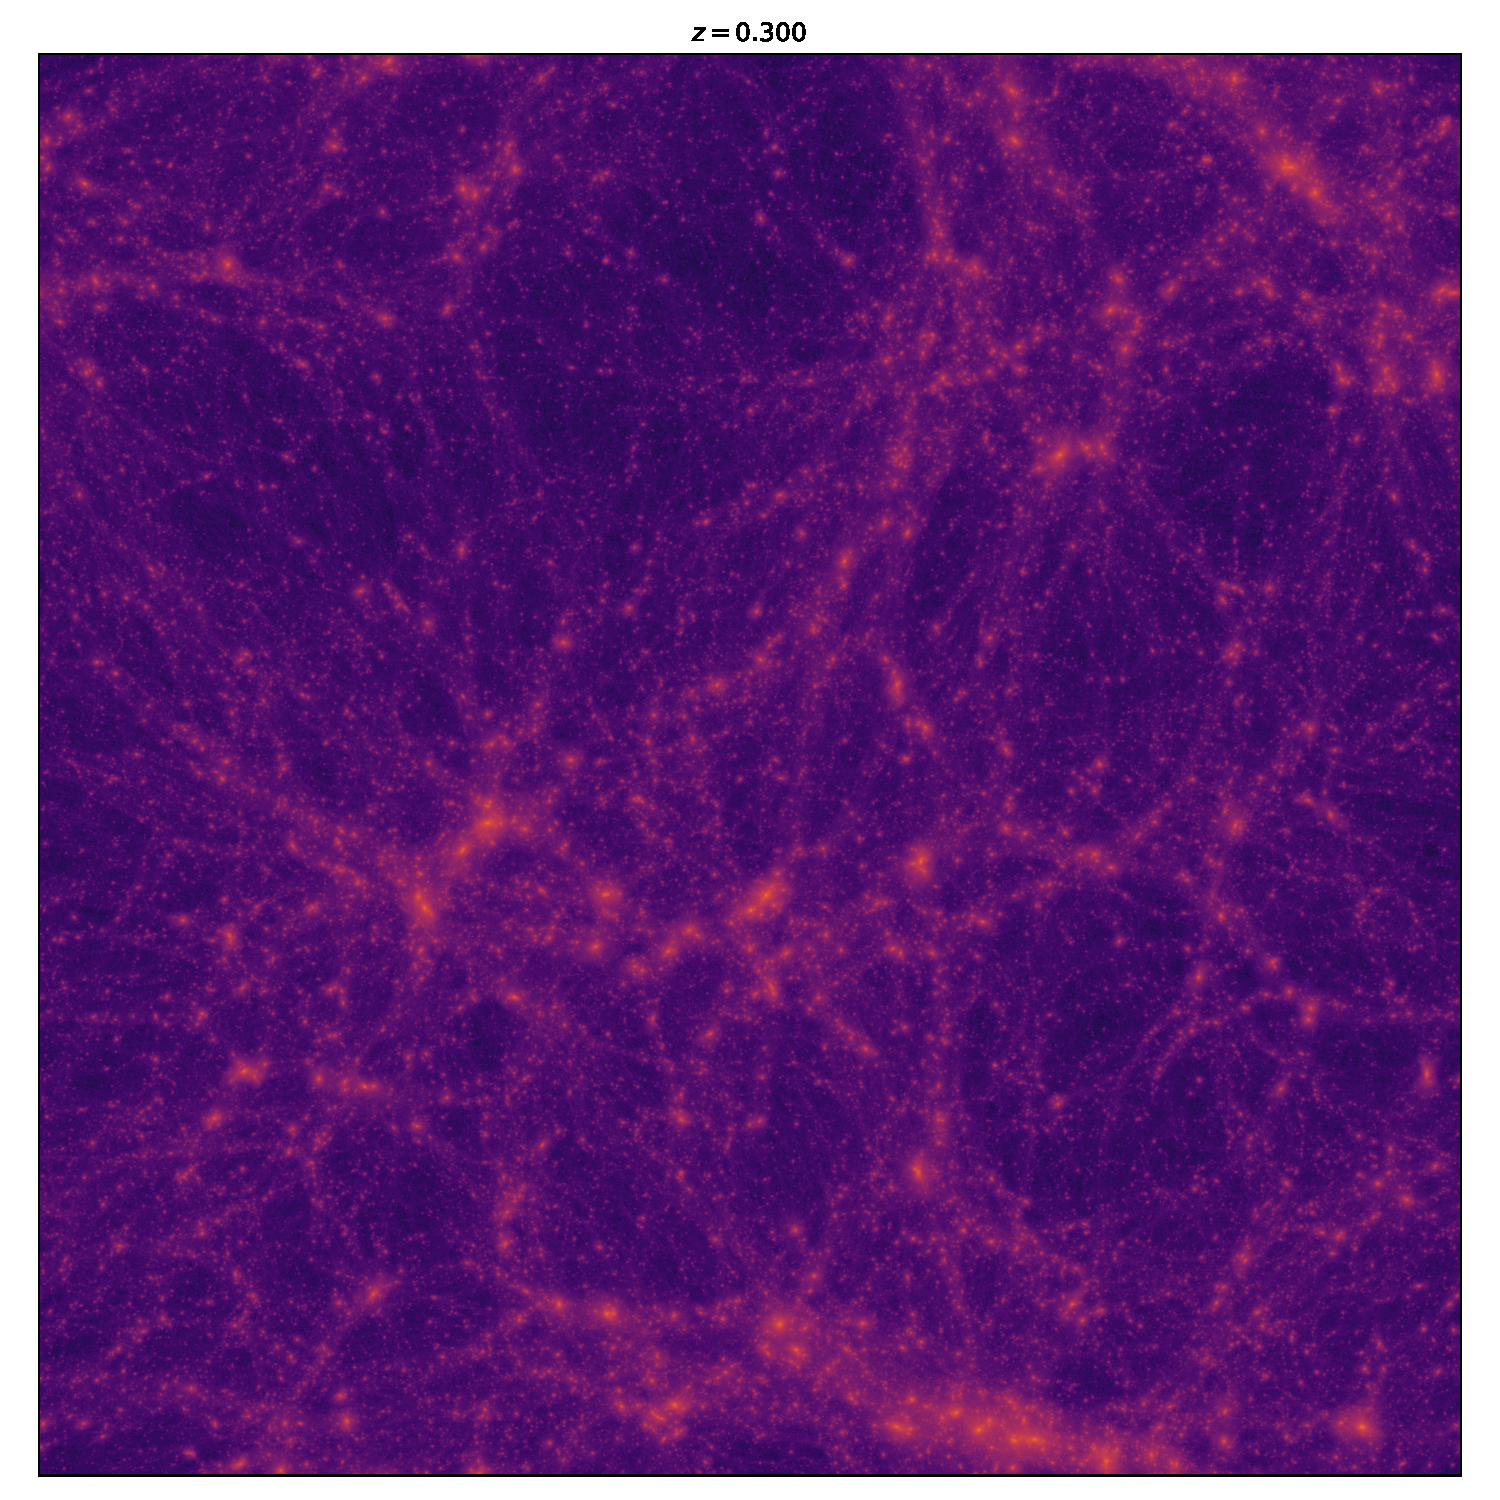
\includegraphics[keepaspectratio,height=\paperheight, width=\paperwidth]{./images/snapshots/particleplot_00032_nolabels.pdf}\hfil}\vfil}}
%    \begin{frame}[plain]
%    \end{frame}
%}
%{
%    \setbeamertemplate{background}
%    {\vbox to \paperheight{\vfil \hbox to \paperwidth{\hfil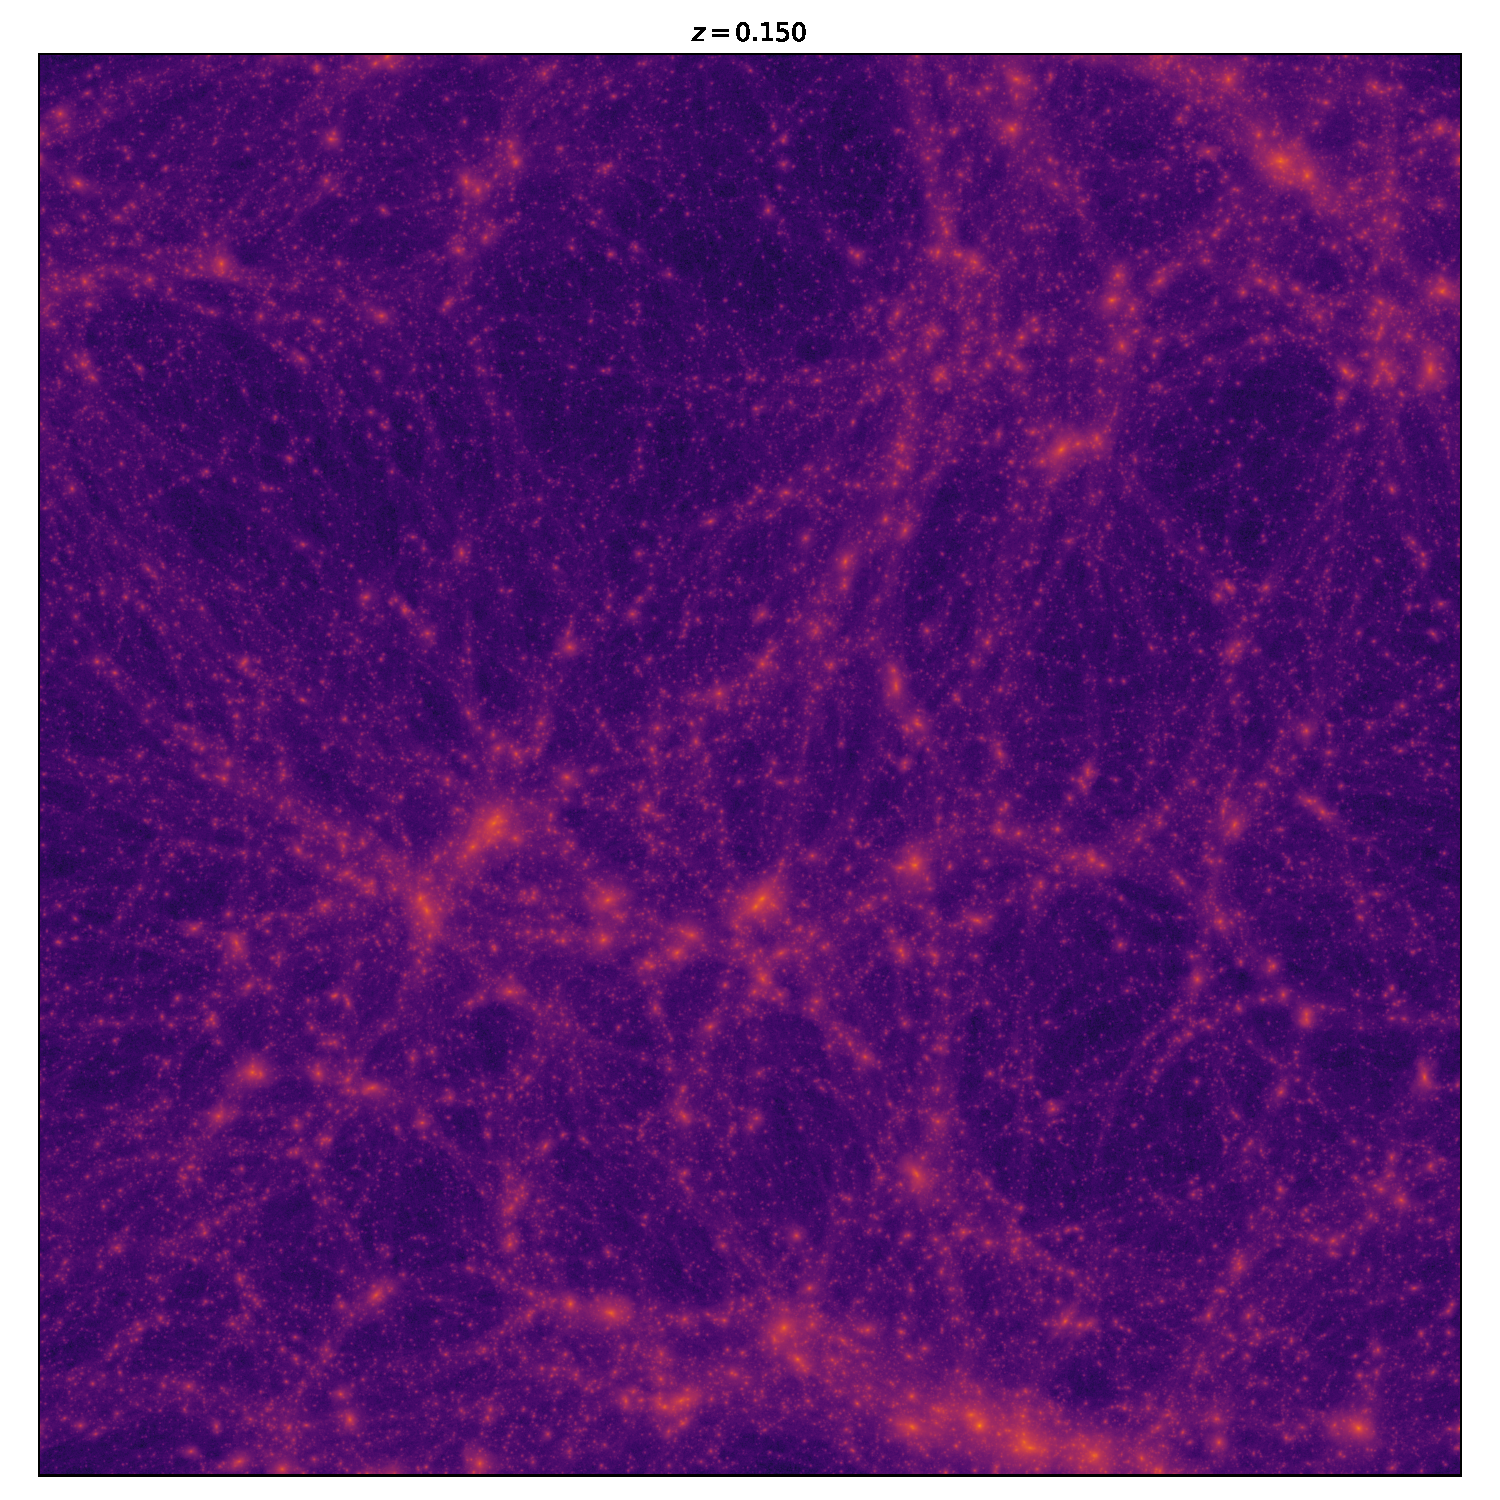
\includegraphics[keepaspectratio,height=\paperheight, width=\paperwidth]{./images/snapshots/particleplot_00035_nolabels.pdf}\hfil}\vfil}}
%    \begin{frame}[plain]
%    \end{frame}
%}
%{
%    \setbeamertemplate{background}
%    {\vbox to \paperheight{\vfil \hbox to \paperwidth{\hfil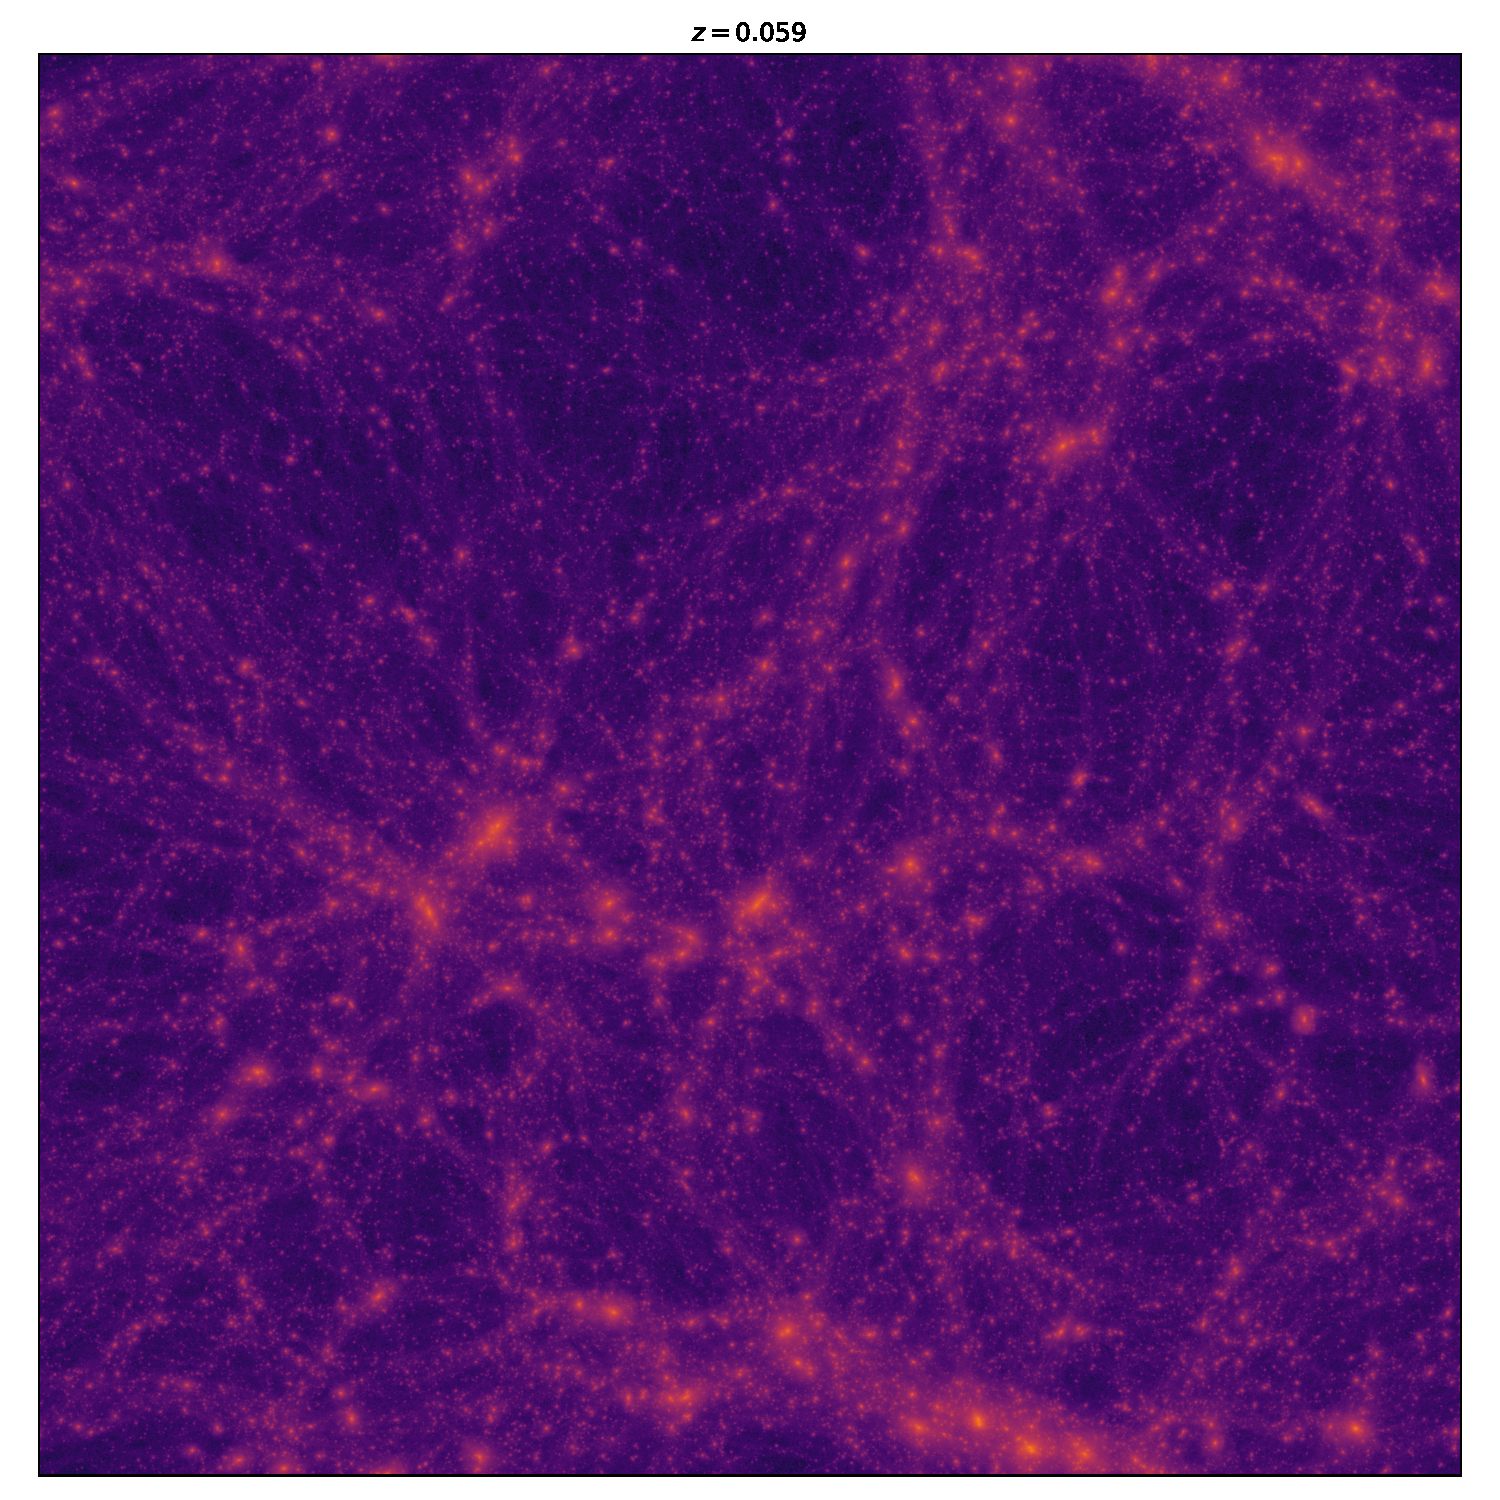
\includegraphics[keepaspectratio,height=\paperheight, width=\paperwidth]{./images/snapshots/particleplot_00038_nolabels.pdf}\hfil}\vfil}}
%    \begin{frame}[plain]
%    \end{frame}
%}
%{
%    \setbeamertemplate{background}
%    {\vbox to \paperheight{\vfil \hbox to \paperwidth{\hfil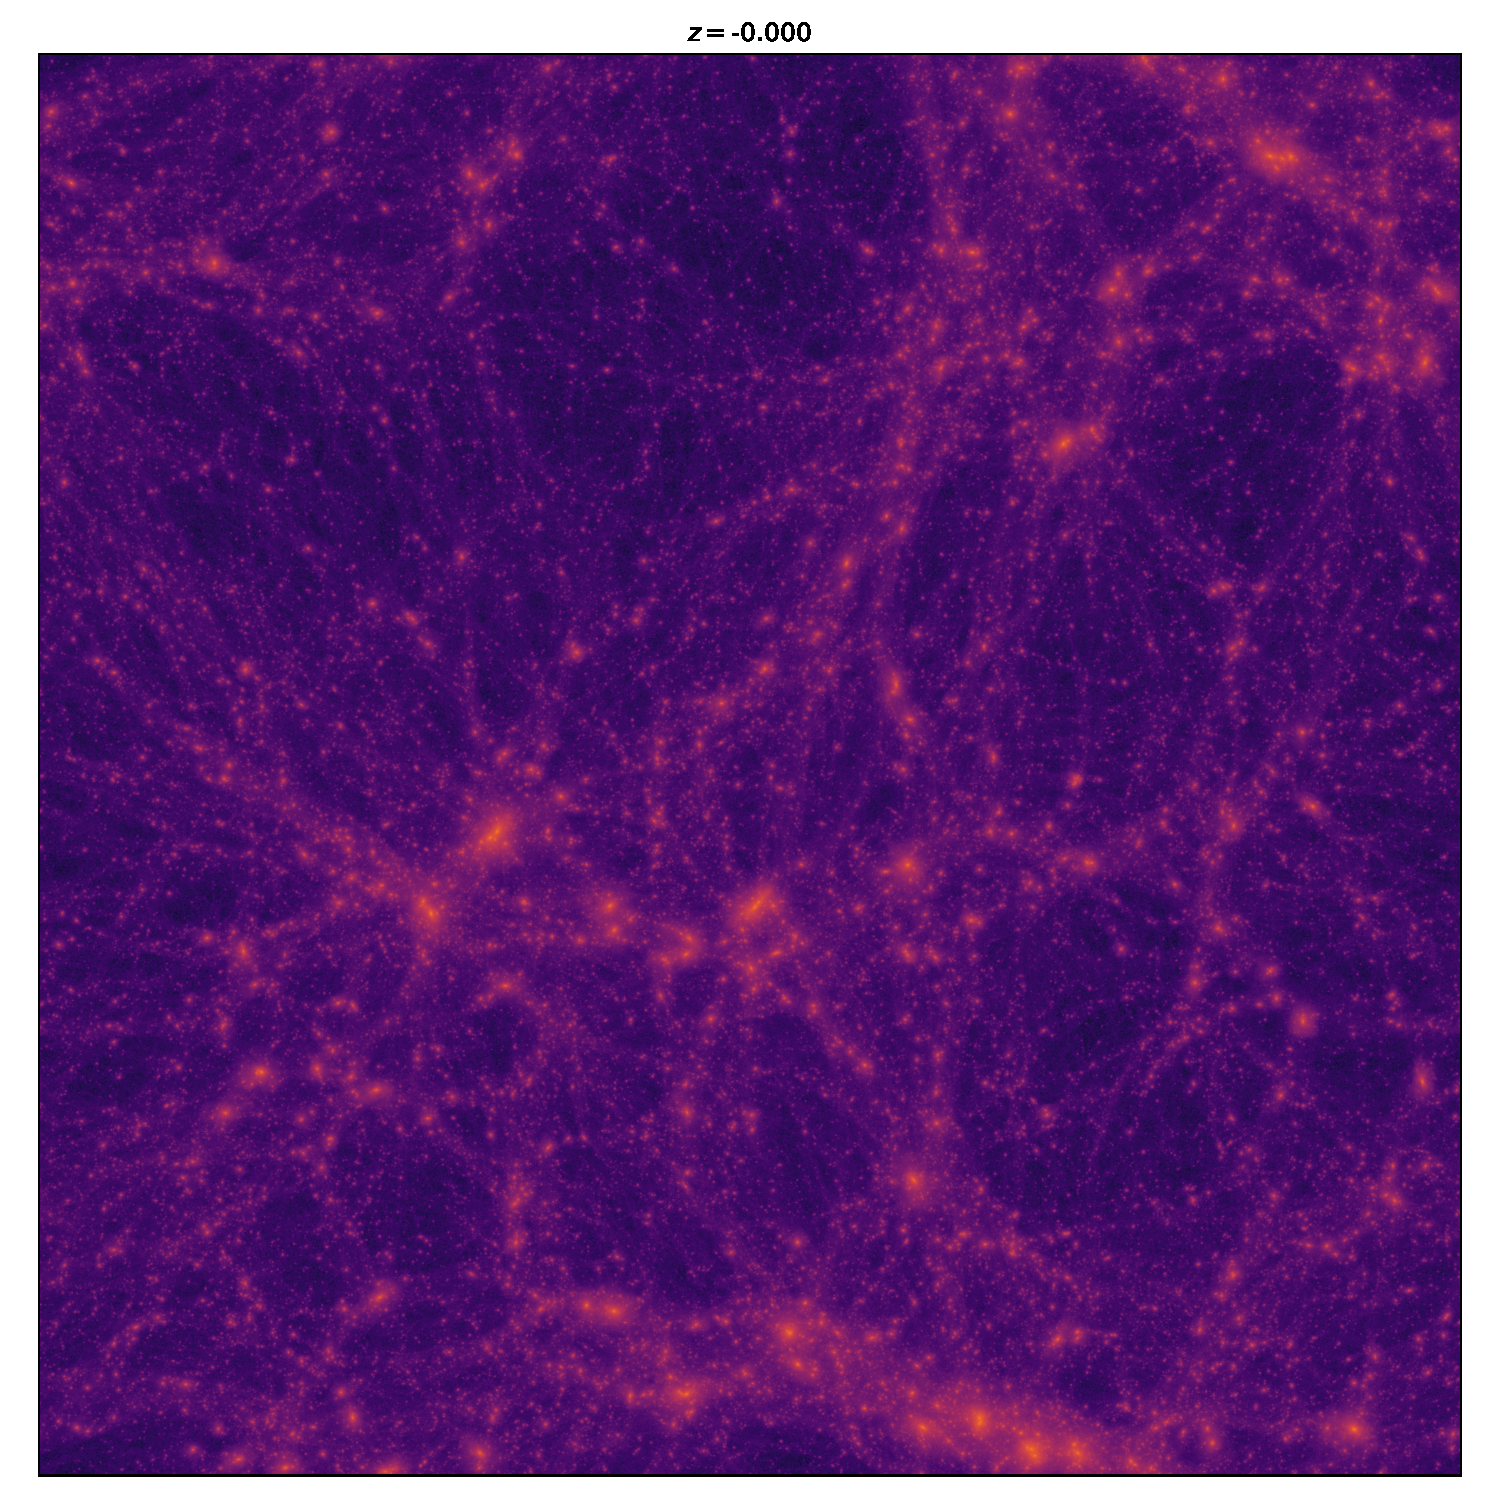
\includegraphics[keepaspectratio,height=\paperheight, width=\paperwidth]{./images/snapshots/particleplot_00041_nolabels.pdf}\hfil}\vfil}}
%    \begin{frame}[plain]
%    \end{frame}
%}
%





\begin{frame}{Making Merger Trees}
    
    How to link progenitors and descendants? 
    
    $\Rightarrow$ trace particles of clumps by their unique particle ID.
    
    In essence: ``in which clumps did particles of a progenitor clump end up in?''
    
    Trace up to a maximal number, $n_{mb}$, of most tightly bound particles of each clump.
    The most tightly bound particles are expected to more likely remain in the same clump in the following snapshot.
    
\end{frame}


\begin{frame}{Making Merger Trees}
        
    To obtain a merger \emph{tree}, as opposed to a merger graph, each progenitor may have exactly one direct descendant clump. 
    Descendants however may have multiple direct progenitors.
    The other direct progenitors of this descendant are then assumed to have merged into the main direct progenitor to form the descendant.
    
    Both progenitors and descendants may have multiple candidates to choose from.
    To identify best progenitor/descendant candidate: Maximise merit function $\mathcal{M}$

\end{frame}


\begin{frame}{Making Merger Trees: Merit Function}
    \begin{equation}
    \mathcal{M}(A,B) = \frac{n_{A \cap B}}{\frac{m_>}{m_<}-1} \label{eq:merit}
    \end{equation}
    
    for each progenitor $A$ and descendant $B$, with $n_{A \cap B}$ = particles both in $A$ and $B$ and $m_>, m_<$ is the bigger or smaller mass between $A$, $B$, respectively.
    
    The factor $(m_>/m_< - 1) ^{-1}$ was chosen to prefer progenitor-descendant pairs of similar mass to avoid strong mass growth fluctuations.
\end{frame}


%\begin{frame}{Making Merger Trees: Fractures}
%    \begin{figure}[H]
%        \centering
%        \includegraphics[width=.5\textwidth]{../report/images/tikz/fracture.pdf}
%    \end{figure}
%    
%    Illustration of a progenitor $A_1$ at time $t_1$ which is partially merged into a descendant $B_1$ at time $t_2 > t_1$, but some other part $B_2$ isn't. 
%    Because $A_1$ is not the main progenitor of $B_1$, by assigning its descendant only according to the merit function \eqref{eq:merit} would not pass on its formation history to $B_2$, but treat it as newly formed.
%    %            The size of the circles represents the haloes' masses, the $x$-axis has no physical meaning.
%    
%    $\Rightarrow$ prefer to link progenitors with any descendant candidate instead of merging it into best candidate
%\end{frame}


\begin{frame}{Making Merger Trees: Jumpers and Orphans}
    
    Galaxies will be placed at the position of the most tightly bound particle of each clump once the merger trees have been obtained.
    
    Once a clump is merged into some descendant, the last identifiable ``galaxy particle'' is tracked as an orphan galaxy in future snapshots.
    
    The orphan galaxy particles are also used to counter failures of the clump finding algorithm: Sometimes substructure is not identified in the density field of a host halo, even though it exists.
    
\end{frame}


{
    \setbeamertemplate{background}
    {\vbox to \paperheight{\vfil \hbox to \paperwidth{\hfil\includegraphics[keepaspectratio,height=\paperheight, width=\paperwidth]{./images/jumper-demo/jumper-demo.pdf}\hfil}\vfil}}
    \begin{frame}[plain]
    \end{frame}
}



%\begin{frame}{Making Merger Trees}
%    Progenitor candidates from adjacent snapshots are preferred to establish a link because they are expected to be more robustly tracked through more than $1$ particle.
%    
%    If a descendant however doesn't have any progenitor candidates, the most tightly bound orphan galaxy particle inside it is taken to be its progenitor from a non-adjacent snapshot, provided such a particle exists.
%\end{frame}



{
    \setbeamertemplate{background}
    {\vbox to \paperheight{\vspace{1.5cm} \hbox to \paperwidth{\hfil\includegraphics[keepaspectratio,height=\paperheight, width=\paperwidth]{../report/images/mergertree.pdf}\hfil}\vfil}}
    \begin{frame}
        \frametitle{Example of a Resulting Mergertree}
        \vspace{6cm}
        \small\texttt{The merger tree of the most massive central halo of a $256^3 \approx 1.7\times 10^7$ particle simulation. 
            The redshift at the time of the snapshot is given on the y-axis, the x-axis has no physical meaning.
%            The tree contains over 1000 branches.
        }
    \end{frame}
}



{
    \setbeamertemplate{background}
    {\vbox to \paperheight{\vspace{1cm} \hbox to \paperwidth{\hfil\includegraphics[keepaspectratio,height=\paperheight, width=0.45\paperwidth]{./images/mergertree_stats/presentation-length_of_main_branch.pdf}\hspace{0.5cm}\includegraphics[keepaspectratio,height=\paperheight, width=0.45\paperwidth]{./images/mergertree_stats/presentation-number_of_branches.pdf}\hfil}\vfil}}
    \begin{frame}
        \frametitle{Tree Statistics}
        \vspace{7cm}
        \setstretch{0.5}
        \small\texttt{Length of main branches and the
            number of branches of $z = 0$ clumps of a $256^3$ particle simulation with $m_p \approx 1.6\times 10^9 \msol$.
        }
    \end{frame}
}




\begin{frame}{What Parameters Give Best Merger Trees?}
    
    The exact definition of a halo and particularly for a subhalo is not unique throughout literature and may depend on the application.
    
    What definition is best for reliable merger trees?
    
    $2$ sets of definitions have been tested:
    \begin{enumerate}
        \item does substructure of subhaloes contribute to subhaloes' mass? (\texttt{inclusive}) or not? (\texttt{exclusive})
        \item Define bound particle: Is it allowed to leave spatial boundary of clump (\texttt{no saddle}) or not? (\texttt{saddle})
    \end{enumerate}

    
\end{frame}





\begin{frame}{What Parameters Give Best Merger Trees? Methods}
      
   \textbf{Logarithmic Mass Growth}
        %
        \begin{align}
            \frac{\de \log M}{\de \log t} \approx \frac{(t_{k+1}+t_{k})(M_{k+1} -M_{k})}{(t_{k+1} - t_k)(M_{k+1} + M_{k})} \equiv \alpha_M(k, k+1)
        \end{align}
        %
        where $k$ and $k+1$ are a clump and its descendant, with masses $M_k$ and $M_{k+1}$ at times $t_k$ and $t_{k+1}$, respectively.
        
        To reduce the range of possible values to the interval $(-1, 1)$, define
        %
        \begin{align}
            \beta_M = \frac{2}{\pi}\arctan(\alpha_M) 
        \end{align}
        %
        $\beta_M \rightarrow \pm 1$ imply $\alpha_M \rightarrow \pm \infty$, indicating extreme mass growth or losses.
\end{frame}


\begin{frame}{What Parameters Give Best Merger Trees? Methods}
    \textbf{Mass Growth Fluctuations}
        \begin{align}
            \xi_M = \frac{\beta_M(k, k+1) - \beta_M(k-1, k)}{2}
        \end{align}
        %
        where $k-1$, $k$, $k+1$ represent consecutive snapshots.
        When far from zero, it implies an extreme growth behaviour. 
        For $\xi_M\rightarrow \pm 1$, $\beta_M(k, k+1) \rightarrow \pm 1$ and $\beta_M(k-1, k) \rightarrow \mp 1$, indicating extreme mass loss followed by extreme mass growth for the upper sign, and the opposite behaviour for the lower sign.

    
    
\end{frame}






{
    \setbeamertemplate{background}
    {\vbox to \paperheight{\vspace{1.5cm} \hbox to \paperwidth{\hfil\includegraphics[keepaspectratio,height=\paperheight, width=\paperwidth]{../report/images/saddle-vs-nosaddle/mass_growth_and_fluctuation.png}\hfil}\vfil}}
    \begin{frame}
        \frametitle{Mass Growth and Mass Growth Fluctuations}
        \vspace{7cm}
        \setstretch{0.8}
        \small\texttt{The distributions are computed as a histogram normalised by the total number of events found throughout the entire simulation.
            Only clumps with masses above $5\times 10^{11} \msol$ were included.
            %            The tree contains over 1000 branches.
        }
    \end{frame}
}
